% !TeX root = ../main.tex

\chapter{系统概要设计}
本章叙述了CI/CD流水线调度系统的设计。
首先介绍了系统的总体设计和架构分层,随后分别叙述系统内各个模块的设计与其之间的连接,
然后后对系统的数据库从概念设计和逻辑设计两方面进行了阐述,最后对本小节内容进行了总结。

\section{系统总体设计}

在对整个CI/CD流水线调度系统进行需求分析后,可以发现本系统的功能业务复杂且对部分服务的横向扩展有着较高需求。
可将本系统的核心模块拆分为三个微服务,分别为Backend服务、调度器服务和执行器服务,每个服务下又包含一些子模块。
进行这样服务划分的目的是降低系统间各模块的耦合性,并为不同的模块分配合适的资源,方便不同的模块分别以多节点的方式进行部署。
同时,拆分后的服务借助容器调度系统Kubernetes,可以实现弹性扩容和故障转移。
系统架构图如图~ \ref{fig:系统架构图}

\begin{figure}[h]
  \centering
  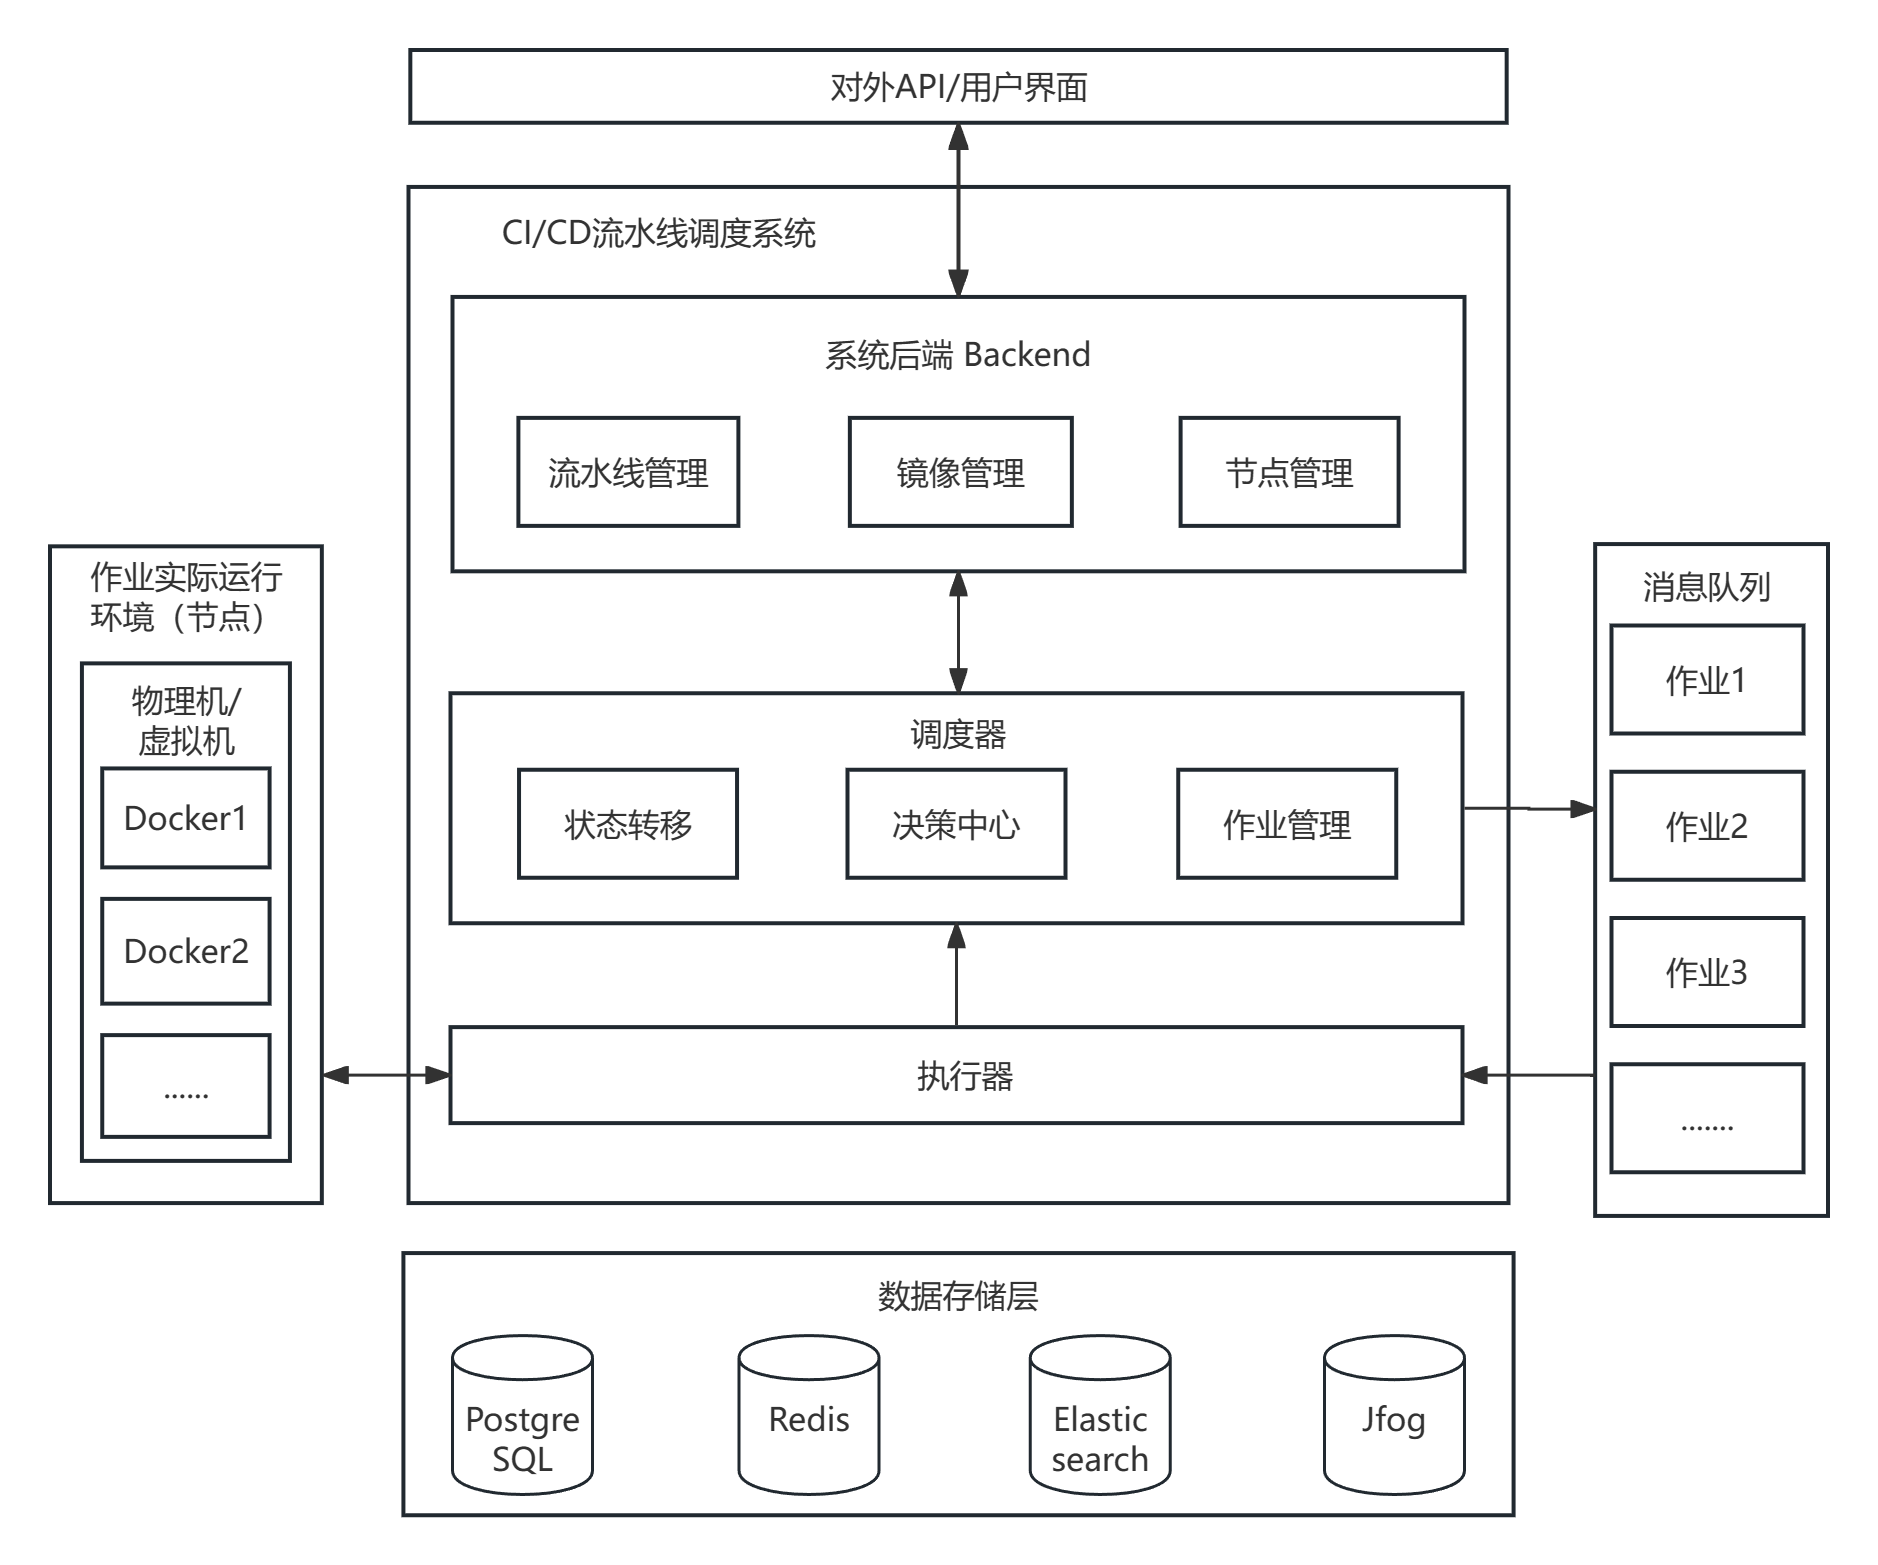
\includegraphics[width=1\textwidth]{流水线系统架构图.png}
  \caption{系统架构图}
  \label{fig:系统架构图}
\end{figure}

首先最上层是对外公开的api和前端UI,用户将通过该层与

系统内部同一时刻将有许多流水线作业同时执行,调度器负责流水线中各个子概念的状态切换,同时依据不同流水线的配置和状态来对当前流水线作业的调度进行决策,将需要被执行的作业交付给执行器模块。
执行器则最终负责各个流水线作业的真实执行,将作业转换为真正的可执行程序或者脚本后在真实的运行环境(Docker、物理机或虚拟机)中执行,并实时监控中运行环境中作业的运行状态,反馈给调度器。



\section{系统模块设计}
把每个模块讲一下:加入数据流图描述作业数据的流动。

\subsection{Backend}

首先是Backend模块,系统通过该模块向外部暴露API以供前端/外部接口调用。
用户在前端进行的操作、填写的配置信息等将通过API接口传递给Backend模块,Backend模块接收到数据后,会进行相应的业务逻辑处理,如对用户创建的流水线进行合法性校验、对作业数据进行合法性校验等,最后负责将数据落库。
同时,在流水线运行过程中,用户对流水线的手动干预操作,也是先调用接口传递给Backend模块,然后再由Backend模块进行一定处理后传递给调度器模块,用户界面与调度器模块完全解耦。

Backend有以下三种典型服务场景:

当用户通过UI界面或API接口传入如“取消”、“跳过”、“人工审核通过”等人工干预命令时,Backend会根据权限模型对用户进行鉴权,如只有流水线的拥有者才有权干预流水线、只有预设的审核人才有权进行人工审核等。
通过鉴权后,Backend将对人工干预命令进行进一步封装,携带一些额外的信息后,将命令发送给调度器模块,由调度器对流水线的执行进行真正的干预。

当用户通过UI界面或API接口创建或编辑流水线时,Backend会对流水线的内容进行解析,并通过序列化器对内容进行合法性校验,然后将流水线以阶段、作业和任务的维度进行分拆,
并将拆解后的流水线数据持久化进数据库。
同样的,用户通过UI界面或API接口进行镜像管理和节点管理时,Backend模块负责业务逻辑处理、数据持久化以及与镜像服务器或节点服务器之间的交互等。

当用户通过UI界面或API接口触发流水线时,Backend将从数据库中获取流水线数据,进行一定封装后发送给调度器模块。
随后,调度器会不断地向Backend返回流水线的执行信息,以便Backend实时更新流水线的运行状态。
与此同时,Backend会接收到前端的轮询请求,用以实时展示给用户。

\subsection{调度器}

调度器模块是整个系统的核心模块,其中包含状态转移、决策中心与作业管理三个子模块,分别介绍如下:

\subsubsection{状态转移}

对流水线、阶段、作业和任务的状态维护至关重要,一来用户需要实时观察流水线中各个子概念的状态,以便实时知晓运行情况;
二来子概念的状态是流水线中进行下一步决策的重要判定依据,例如只有一个阶段中的所有作业都被置为成功,阶段的状态才会变为成功,只有当阶段被置为成功,且下一个阶段是准入的,才会触发写一个阶段的执行。
依据需求分析,结合对目前市面常见CI/CD平台的参考,系统中设计了就绪中(Pending)、执行中(Running)、执行成功(Success)、执行失败(Failed)、被跳过(Skipped)、被取消(Canceled)六种状态。
各个状态的具体解释如表~\ref{tab:状态解释表}。
\begin{table}[h]
  \centering
  \caption{状态解释表}
  \label{tab:状态解释表}
  \begin{tabular}{cl}
    \toprule
    状态           & 解释                                     \\
    \midrule
    就绪中         & 一切准备工作就绪,等待被自动执行、手动执行或审核通过\\
    执行中         & 正在被执行                 \\
    执行成功       & 顺利执行完毕后的状态        \\
    执行失败       & 执行过程中出错后的状态       \\
    被跳过         & 被用户人为干预执行“跳过”后的状态         \\
    被取消         & 被用户认为干预执行“取消”后的状态         \\
    \bottomrule
  \end{tabular}
\end{table}
以上状态适用于流水线中的各个子概念。

引起一个作业状态转移来自于两种事件,一种是来自Backend的人工干预事件,一种是执行器通知的作业成功或失败的事件。
这种根据事件或动作引起状态转移的情况,在软件工程中可以使用有限状态机(Finite State Machine,FSM)的模型来设计。
根据有限状态机的理论,我们需要识别模型中的“状态”和“事件”,状态已经在前文有所定义了,而对于作业(Job)来讲:事件则包含所有的人工干预操作:
触发、取消、跳过和重试,同时包含执行器的状态通知:成功和失败,其次还应包含人工审核的相关内容,包含审核通过和审核驳回。

作业状态机状态转移如表~\ref{tab:作业状态机状态转移表}所示。

\begin{table}[h]
  \centering
  \caption{作业状态机状态转移表}
  \label{tab:作业状态机状态转移表}
  \begin{tabular}{cll}
    \toprule
    事件           & 允许该事件的状态          & 事件发生后状态                  \\
    \midrule
    触发           & 就绪中                   & 执行中       \\
    取消           & 执行中                   & 被取消       \\
    跳过           & 执行中                   & 被跳过       \\
    重试           & 执行失败、被跳过、被取消   & 执行中       \\
    审核通过        & 就绪中                   & 执行中        \\
    审核驳回        & 就绪中                   & 执行失败       \\
    作业执行成功     & 执行中      & 执行成功   \\
    作业执行失败     & 执行中      & 执行失败   \\
    作业执行超时     & 执行中      & 执行失败   \\
    \bottomrule
  \end{tabular}
\end{table}

对于任务(Task)而言,其状态变化与作业类似,但区别在于作业时用户操作和执行器执行的最小单位,
而任务是包含于作业之中的子概念,所以当用户事件导致作业的状态发生变化时,其中任务的状态也随之改变。
例如,当用户跳过一个执行中的作业时,作业的状态应被设为被跳过,同时作业内所有的任务的状态将全部被设为被跳过,对于重试、取消、触发、审核通过和审核驳回事件同理。
而执行成功和执行失败事件来说则有所不同,由于作业中的任务是顺序执行的,所以任务与任务之间有执行的前后之分,故并不能统一进行状态修改。
对于任务来讲,执行器会独立地触发任务执行成功与任务执行失败两种事件,这是因为任务所执行的脚本本质上是整个作业所执行脚本的片段,执行器能够感知到目前已经执行的脚本是否执行成功,所以这两种事件能够独立于作业的成功与失败之外引发任务的状态变动。

任务状态机状态转移如表~\ref{tab:任务状态机状态转移表}所示。

\begin{table}[h]
  \centering
  \caption{任务状态机状态转移表}
  \label{tab:任务状态机状态转移表}
  \begin{tabular}{cll}
    \toprule
    事件           & 允许该事件的状态          & 事件发生后状态                  \\
    \midrule
    所属作业被触发           & 就绪中                   & 执行中       \\
    所属作业被取消           & 执行中                   & 被取消       \\
    所属作业被跳过           & 执行中                   & 被跳过       \\
    所属作业重试            & 执行失败、被跳过、被取消   & 执行中       \\
    所属作业审核通过        & 就绪中                   & 执行中        \\
    所属作业审核驳回        & 就绪中                   & 执行失败       \\
    任务执行成功            & 执行中      & 执行成功   \\
    任务执行失败            & 执行中      & 执行失败   \\
    作业执行超时            & 执行中      & 执行失败   \\
    \bottomrule
  \end{tabular}
\end{table}

对于阶段(stage)而言,其状态变换完全不受执行器的影响,因为执行器执行的是作业,而阶段本质上只是一套可以并行的作业的逻辑集合,
所以阶段的状态仅由该阶段中的所有作业的状态共同决定。
一般来说,我们期望阶段中最值得关注的作业状态成为整个阶段的状态,同时需要结合不同状态的特性,来设计阶段的状态转移。
,为了统一阶段状态处理逻辑,系统中引入了“状态优先级”这一概念,系统中不同状态的优先级如表\ref{tab:状态优先级表}所示。

\begin{table}[h]
  \centering
  \caption{状态优先级表}
  \label{tab:状态优先级表}
  \begin{tabular}{cl}
    \toprule
    状态           & 优先级                                     \\
    \midrule
    被跳过         & 1         \\
    执行成功       & 2         \\
    就绪中         & 3         \\
    执行中         & 4         \\
    被取消         & 5         \\
    执行失败       & 6         \\
    \bottomrule
  \end{tabular}
  \note{注:数字越大表示优先级越高}
\end{table}

当一个阶段内的任意作业的状态发生变化时,系统会将本阶段内所有作业状态中的状态优先级最高的状态设置为阶段的状态。
比如,某阶段中有三个作业,作业1和作业2处于执行成功的状态,作业3的状态为执行中,所以该阶段的状态应是优先级最高的作业3的状态,也为执行中,
这是符合逻辑的,因为阶段内存在尚未执行完的作业,所以整个阶段的状态理应处于执行中;
又比如作业1和作业2被跳过,作业3处于执行成功的状态,则整个阶段的状态为执行成功,这是因为用户跳过一个作业,说明用户并不关注该作业的执行,故赋予其最低优先级。
其余情况均可参照表\ref{tab:状态优先级表}进行判断。
系统通过这种阶段优先级的处理方式,极大简化了阶段的状态转移逻辑。
流水线的状态转移与阶段类似,根据流水线下所有阶段状态的最高优先级来确定流水线的状态,具体内容不再赘述。

\subsubsection{决策中心}
决策中心依据当前Backend传入的命令以及目前流水线中作业与任务的状态,来准确地生成事件以及事件相关活动,以下一一介绍各种事件的产生条件以及活动设计。

\paragraph{触发作业}
触发作业事件存在两种产生时机,一种是调度器收到来自Backend的触发流水线命令时,决策中心会对首个阶段中的作业一一进行处理;
另一种情况是,当一个阶段状态变更为取消或成功时,会对当前阶段的下一阶段中的所有作业进行处理。

此时需要进行一些条件判断,首先需要判断阶段和作业的准入条件,如果是自动触发,则进行下一步;
如果是手动触发,则需要等待Backend端传来手动触发阶段和作业的命令。
一旦准入条件满足,即可将作业交付给作业管理子模块,由作业管理子模块将作业交付给执行器,待执行器执行作业。

注意,以上条件满足时并不会立即产生触发作业事件,因为执行器的并行处理作业是有数量上限的,当执行器已经达到满载,多余的作业会堆积在消息队列待执行器拉取,
所以只有当决策中心收到执行器报告的执行信息时,才会发出触发作业事件。触发作业时序图如图\ref{}所示。

\begin{figure}[h]
  \centering
  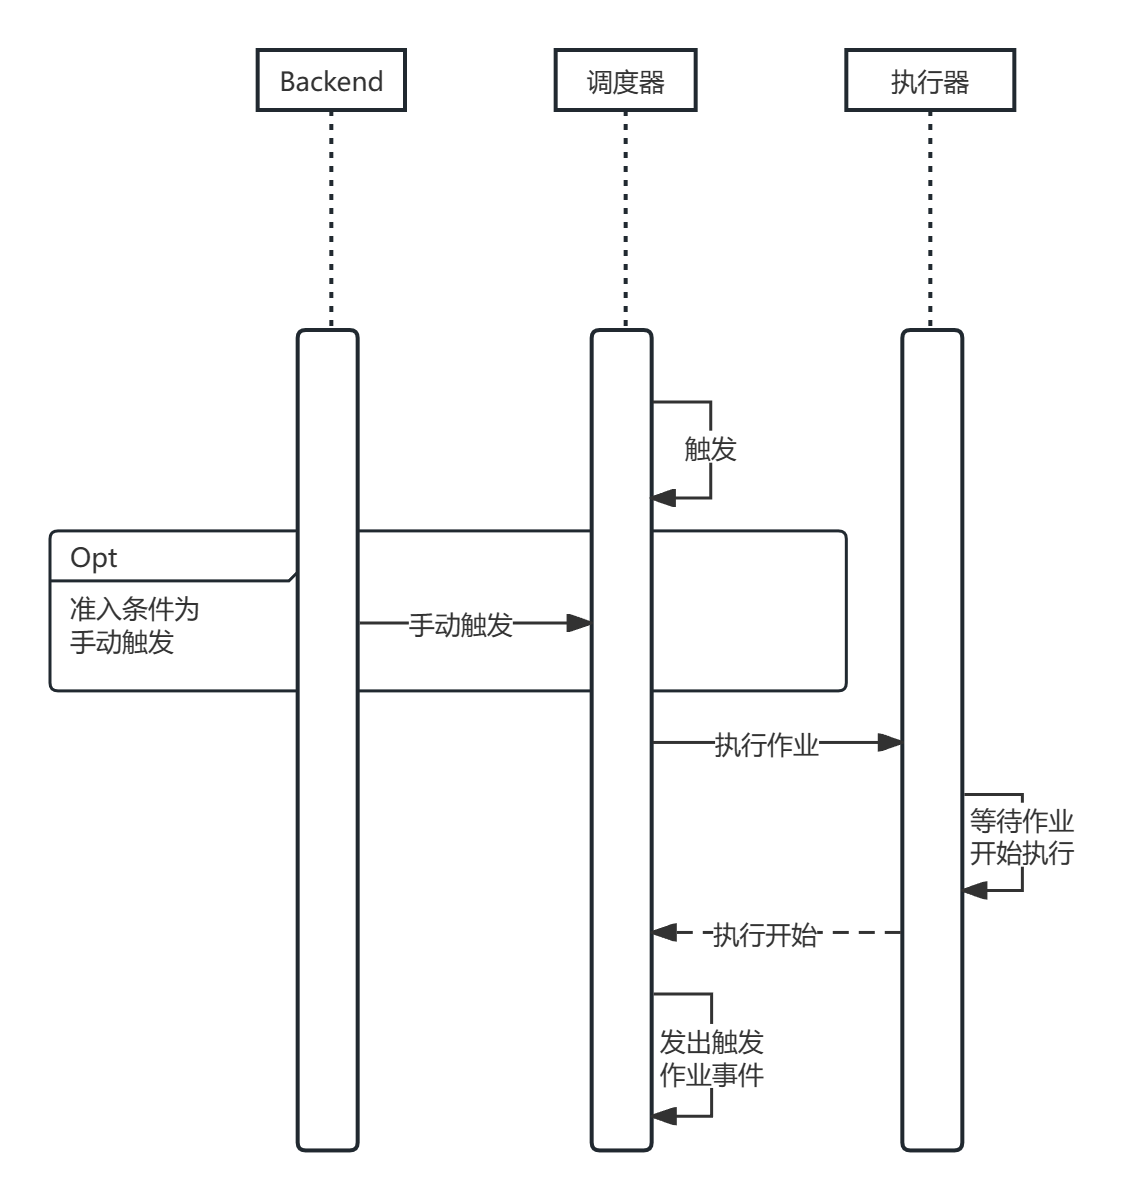
\includegraphics[width=0.8\textwidth]{触发作业时序图.png}
  \caption{触发作业时序图}
  \label{fig:触发作业时序图}
\end{figure}

\paragraph{跳过作业与取消作业}
在决策中心层面,跳过作业与取消作业的活动类似,只不过转移后的状态不同。
当决策中心收到Backend发出的跳过或取消作业的命令时,首先判断任务状态是否为执行中,只有任务状态为执行中时才允许跳过与取消。
然后决策中心将发出跳过或取消事件交由作业状态机进行状态流转,此后需要调度器主动向执行器发出一个中止作业的命令,避免执行器继续执行作业,浪费系统资源。

跳过作业与取消作业时序图如图\ref{}所示。

\begin{figure}[h]
  \centering
  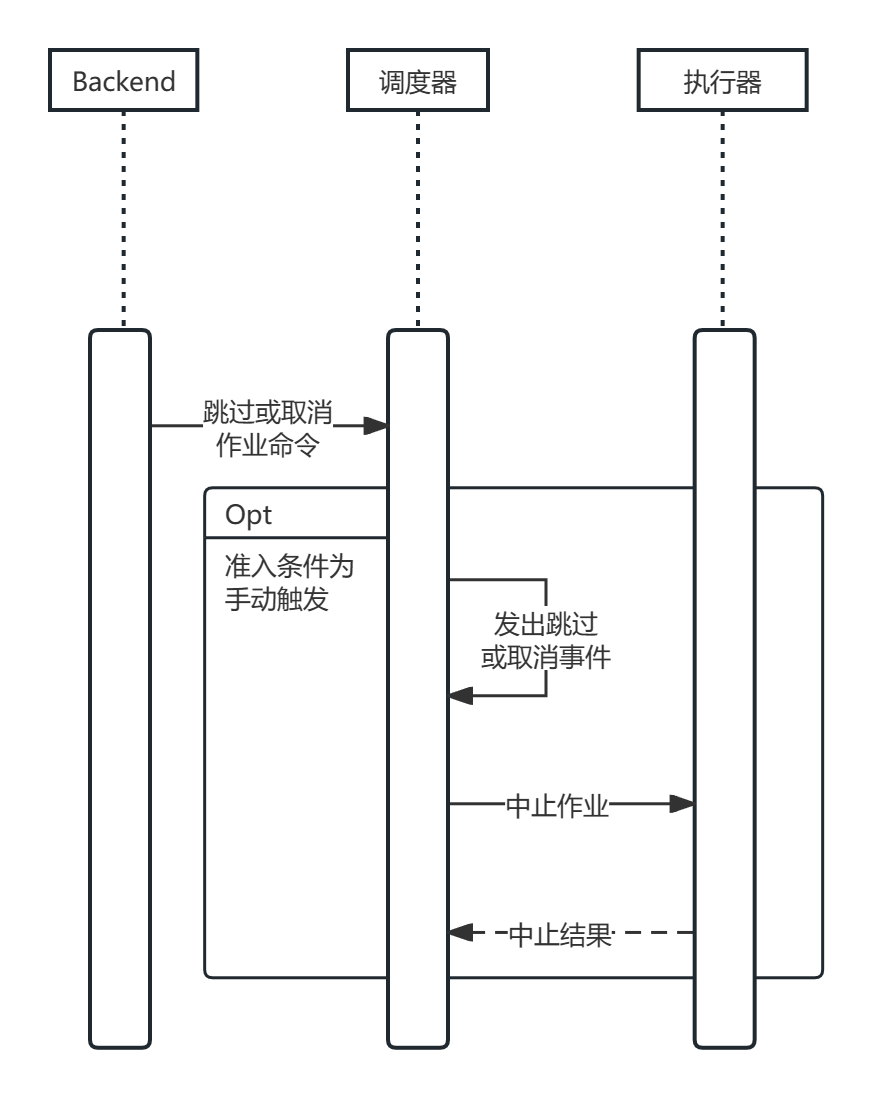
\includegraphics[width=0.8\textwidth]{跳过或取消作业时序图.png}
  \caption{跳过或取消作业时序图时序图}
  \label{fig:跳过或取消作业时序图}
\end{figure}

\paragraph{执行成功与执行失败}
执行失败与执行失败的活动本质上也是类似的,这一事件都是由执行器通知调度器而产生。
当执行器在实际运行环境中检测到作业中任务的脚本执行完毕后,将发送通知调度器的决策中心模块,
同理当执行器在实际允许环境中检测到作业的脚本作业中任务的脚本执行完毕后,将发送任务与整个作业失败的通知给调度器。
决策中心受到通知后,将直接产生执行成功或执行失败的事件,不产生额外的活动,接下来交由调度器进行状态转移。

\subsubsection{作业管理}
该子模块面向Backend对作业进行了二次封装和管理,包括提交作业、获取作业、操作作业,并且接收流水线执行器的作业获取请求和作业执行结果上报,还需要处理作业超时等。

首先,作业管理模块负责将决策中心传来的作业信息进行封装,创建作业实例。每个作业实例包含了执行该作业所需的所有信息,如执行脚本、环境变量和内部各个任务的脚本等。这些信息是执行器执行作业以及后续作业管理的基础。

针对每个作业的执行,作业管理模块都会根据传入的超时时间设定一个超时监控机制。
一旦作业开始执行,计时开始,如果作业执行时间超过了设定的超时时间,作业管理模块将自动触发作业的超时处理活动,中断当前执行的作业,并将触发执行失败事件。
调度器中存在一个检查超时的定时任务,这一定时任务每10秒会检查所有正在执行中的作业,根据作业的开始时间与当前时间计算作业的执行时间,并判断是否超过了预设的超时时间,如果超过了则对超时任务发出执行失败的事件,
同时通知执行器中止作业,避免继续占用资源。
超时处理是确保系统资源不被长时间占用的关键机制,有助于提高系统的整体效率和响应能力。

\subsection{执行器}

执行器的设计目的是为了能够稳定高效地执行不同类型的作业,以待执行的作业信息为输入,以作业执行结果为输出,并且支持快速横向扩展,提高作业执行能力。
作业执行器首先需要能够根据自身能够执行的作业类型获取与之相对应的作业。
获取作业之后,能够保证顺利且高效的完成作业执行。
在执行过程中,将作业内任务的状态上报给调度器;执行完毕后,将作业状态上报给调度器。
执行器本系统将使用开源的Gitlab Runner,GitLab Runner在Gitlab的CI/CD模块中也扮演执行器的功能,并且与Gitlab主模块使用Http Apis进行通信,本系统中将对这些Http Apis进行抓包,获得这些Api的Url以及出入参后,便可如法炮制地将本系统的调度器接入GitLab Runner。
为了保证系统的稳定性,流水线执行器将部署在Kubernetes中,流水线执行器可以根据当前CI/CD的资源需求自动创建或删除副本(在Kubernetes称作Pod),以适应负载的变化:当系统进入使用高峰期时,系统可以自动创建更多的执行器副本来处理请求,而当负载减少时,多余的副本会被自动删除,从而实现资源的高效利用;
同时,当某个执行器发生故障时,Kubernetes会自动检测到故障,并将受影响的CI/CD负载迁移到其他健康的执行器副本上,避免应用程序中断或停止对外提供服务,提高系统稳定性。

\subsection{消息队列}

本系统调度器与执行器之间的消息交互是借助一个消息队列来完成的,本系统中使用阿里巴巴开发的RocketMq 5.0。
当调度器封装好一个流水线作业运行实例时,调度器将作为消息队列的生产者,将作业运行实例放入队列中;执行器作为消息队列的消费者,将持续消费队列中的消息。
调度器和执行器分别与消息队列进行交互,两者之间解耦,便于后续扩展。

系统引入消息队列的主要目的是实现需求分析中的\nameref{subsec:流水线作业合理调度需求}。
首先,消息队列先进先出的特性能够保证执行器有序地消费作业运行实例,避免了程序异步执行带来的作业执行顺序错乱问题,使得作业的执行严格按照调度器预设的顺序执行。
并且,当系统使用高峰期来临,作业量超过了执行器的负载能力时,消息队列承担了缓冲的作用,来不及被消费的作业将按照顺序被堆积在消息队列中,等到执行器处理完当前作业,具备处理能力后,再去消息队列的队头中拉取作业。

调度器、执行器与消息队列之间的时序图如图\ref{fig:消息队列时序图}

\begin{figure}[h]
  \centering
  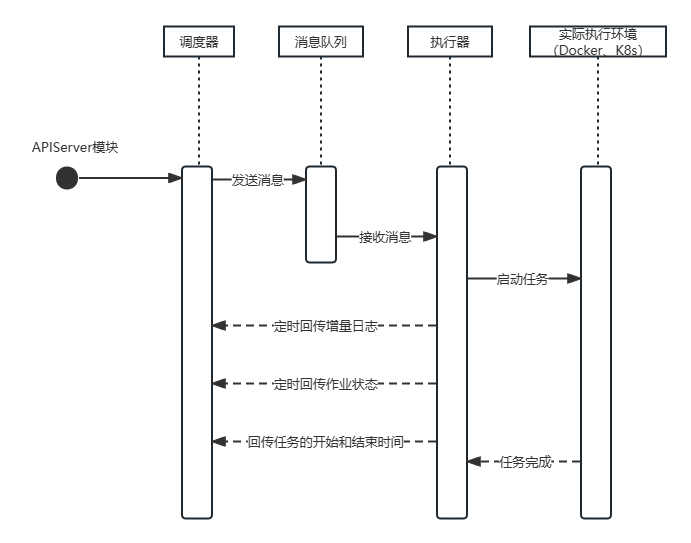
\includegraphics[width=0.8\textwidth]{消息队列时序图.png}
  \caption{调度器、执行器与消息队列间时序图}
  \label{fig:消息队列时序图}
\end{figure}

\subsection{数据存储层}
数据存储层是对本系统中各个数据和文件存储服务的抽象,负责整个系统所有数据的持久化服务。
包括流水线以及其子概念的配置信息、运行记录、Docker镜像、作业执行产物(如编译后压缩产生的tar包等)以及作业运行日志等。

本系统中,使用PostgreSQL存储流水线的配置和运行记录的相关数据,这部分数据属于结构化数据,数据字段和格式较为固定,故采用业界主流的关系型数据库进行存储和管理;
使用Redis存储缓存信息,加快接口的响应速度,提升用户体验;
JFrog Artifactory存储镜像管理模块涉及到的Docker镜像,以及流水线任务执行完成后的执行产物,比如单元测试报告等;
日志平台建立在 Elastic Search 之上,用于集中记录整个系统的所有运行日志,所有子系统的日志都会传送至该平台进行聚合。
其具体原理与功能与本系统主体功能无关,不再赘述。

上述不同类型的数据及其存储方式总结如表\ref{tab:系统数据存储方式}所示.

\begin{table}[h]
  \centering
  \caption{系统数据存储方式}
  \label{tab:系统数据存储方式}
  \begin{tabular}{clll}
    \toprule
    数据类型 & 主要内容      & 存储方式   & 选型 \\
    \midrule
    结构化数据     & 配置信息和运行记录      & 关系型数据库   & PostgreSQL       \\
    缓存数据       & 接口响应数据                   & 键值存储   & Redis       \\
    二进制数据     & Docker镜像、流水线任务执行产物  & 二进制数据管理系统   & JFrog Artifactory   \\
    日志数据       & 日志                & 分布式日志系统  & Elastic Search       \\
    \bottomrule
  \end{tabular}
\end{table}

\section{系统功能设计}

从功能角度,Backend包含以下三个功能模块:流水线管理、镜像管理和节点管理,
其中流水线管理是系统的主体功能,镜像管理以及节点管理服务与流水线作业的环境构建与实际运行。
下文将分别介绍其主要功能设计,系统功能模块图如图~\ref{fig:功能模块图} 所示。

\begin{figure}[h]
  \centering
  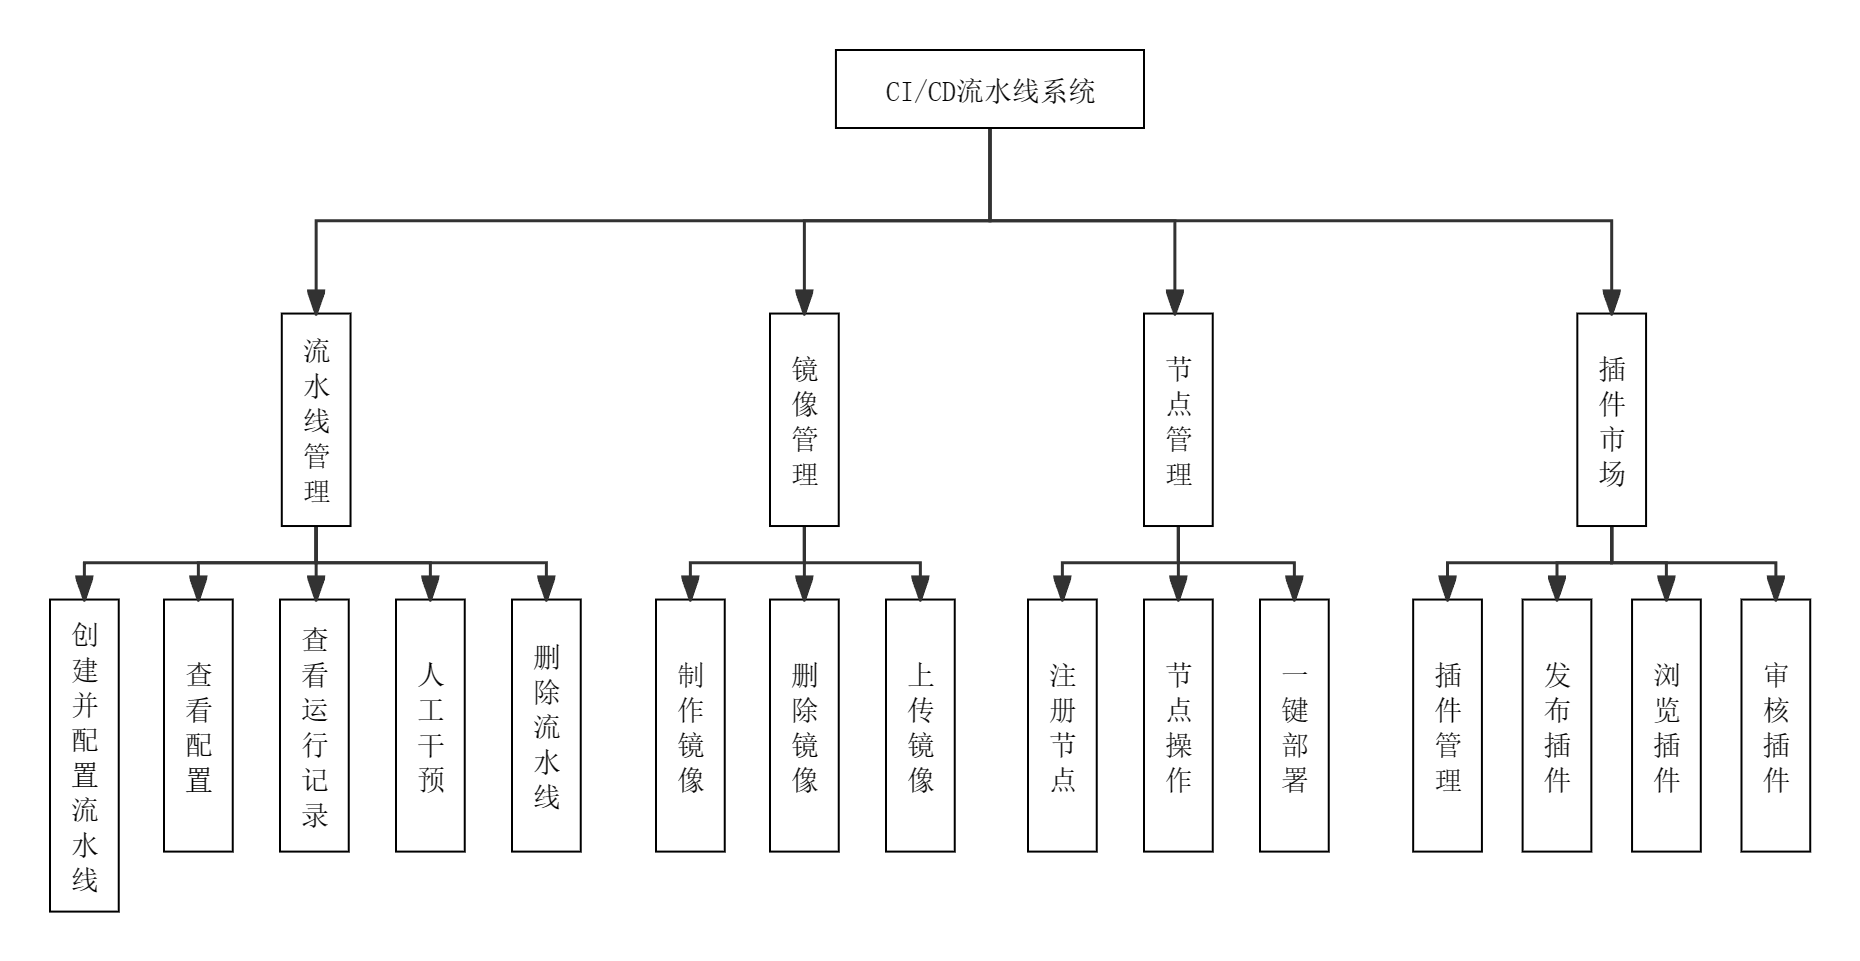
\includegraphics[width=1\textwidth]{功能模块图.png}
  \caption{功能模块图}
  \label{fig:功能模块图}
\end{figure}

\subsection{流水线管理}

流水线管理不仅包括流水线,还包括阶段、作业和任务共四个概念实体,这些实体组成了流水线的拓扑结构。
该模块主要提供了对流水线的基本操作,包括对流水线的增删改查(其中包含了阶段、作业和任务的增删改查)以及流水线的触发。
以下介绍流水线管理中几个关键功能的设计:

\subsubsection{创建并配置流水线}
用户创建流水线时,

\subsubsection{触发流水线}
流水线触发是一套链路复杂的操作,由Backend模块开始触发,涉及到调度器模块、执行器模块和消息队列之间的协同。
首先将递归地创建当前流水线中的所有的阶段、作业与任务的运行记录,并进行数据持久化。
此后Backend模块将把当前流水线的结构与配置转化发送给调度器,调度器中的作业中心会将作业的配置和结构进行解析和二次封装,
待决策中心进一步发出触发的指令后,作业中心会将作业塞入消息队列中待执行器获取。
执行器一旦获取到作业,便会控制作业在实际运行环境中的具体执行。

以上步骤均完成后,流水线才被真正触发,流水线中的第一个作业将会在节点中真正执行。

\subsection{镜像管理}
\label{subsec:镜像管理}

在基于容器的CI/CD系统中,镜像是构建容器的基础。
在本系统中,如果用户定义一个作业为容器类型时,首先需要选择一个镜像,作业执行时本系统的执行器会根据镜像来创建环境,然后在环境中执行作业中的各个任务。
为保证系统中的容器可以满足不同开发、测试和运维人员人员的需要,系统中应确保有足够多种类的镜像提供给用户选择,所以镜像管理在本系统中至关重要。

在为了实现镜像管理,系统底层区分并提供了两种主要的服务:一是负责存储镜像的仓库服务,二是负责创建镜像的构建服务。
仓库服务负责对镜像文件进行检索和清除,而构建服务则承担着容器运行和镜像创建的职责。
通过这两类服务的协同工作,实现了高效的镜像管理。

以下介绍镜像管理中几个关键功能的设计:

\subsubsection{镜像创建}

该环节生产的镜像将在创建流水线作业的时候所使用,作为流水线作业的初始环境。
一般来讲,镜像的构建需要管理员直接操作物理服务器,通过手动输入Docker命令来完成,这一过程不仅繁琐而且存在安全风险。
在本系统中,镜像的创建过程被移到了在线平台上,用户可以通过Web界面进行镜像创建。系统支持以下两种方式:
\begin{enumerate}
  \item 通过DockerFile文件。这是最常见的构建镜像的方法,用户需要在系统中按照特定语法编写DockerFile,其中可以指定基础镜像、构建命令、端口暴露、文件挂载等。
  这要求用户对DockerFile的编写的语法规则以及shell脚本有所了解。
  \item 通过Commit操作。该方法允许将运行中的容器状态保存为新镜像,此过程中需要基于一个初始镜像启动容器,然后进行环境配置,最终提交更改为新镜像。
\end{enumerate}

这两种方法提供了不同的优势和选择灵活性。其中通过Commit操作的方式需要在用户界面中远程连接到容器,这需要借助基于网页的SSH组件(如Wetty、Guacamole、GateWay等)实现,
本系统中使用Wetty实现用户在Web端与容器内部的交互。

当用户制作镜像时,首先需要填写镜像基础信息,如镜像名、标签等,然后Backend模块会检查数据库中是否有冲突的镜像,如果有则重新返回上一步进行填写。
接下来需要用户选择制作方式,如果用户选择Dockerfile方式,则可以在线编写Dockerfile文件或者直接上传文件,然后镜像制作服务器将调用docker build命令来构建镜像,并返回镜像构建结果;
如果用户选择commit方式,则需要用户选择一个基础镜像,镜像服务器将根据基础镜像调用docker run启动一个容器实例,并暴露出SSH服务的端口,用户在前端通过Wetty进入容器后,进行一系列操作后,
服务器中将调用docker commit将该容器提交为镜像。

镜像制作的活动图如图~\ref{fig:镜像制作活动图}所示。

\begin{figure}[h]
  \centering
  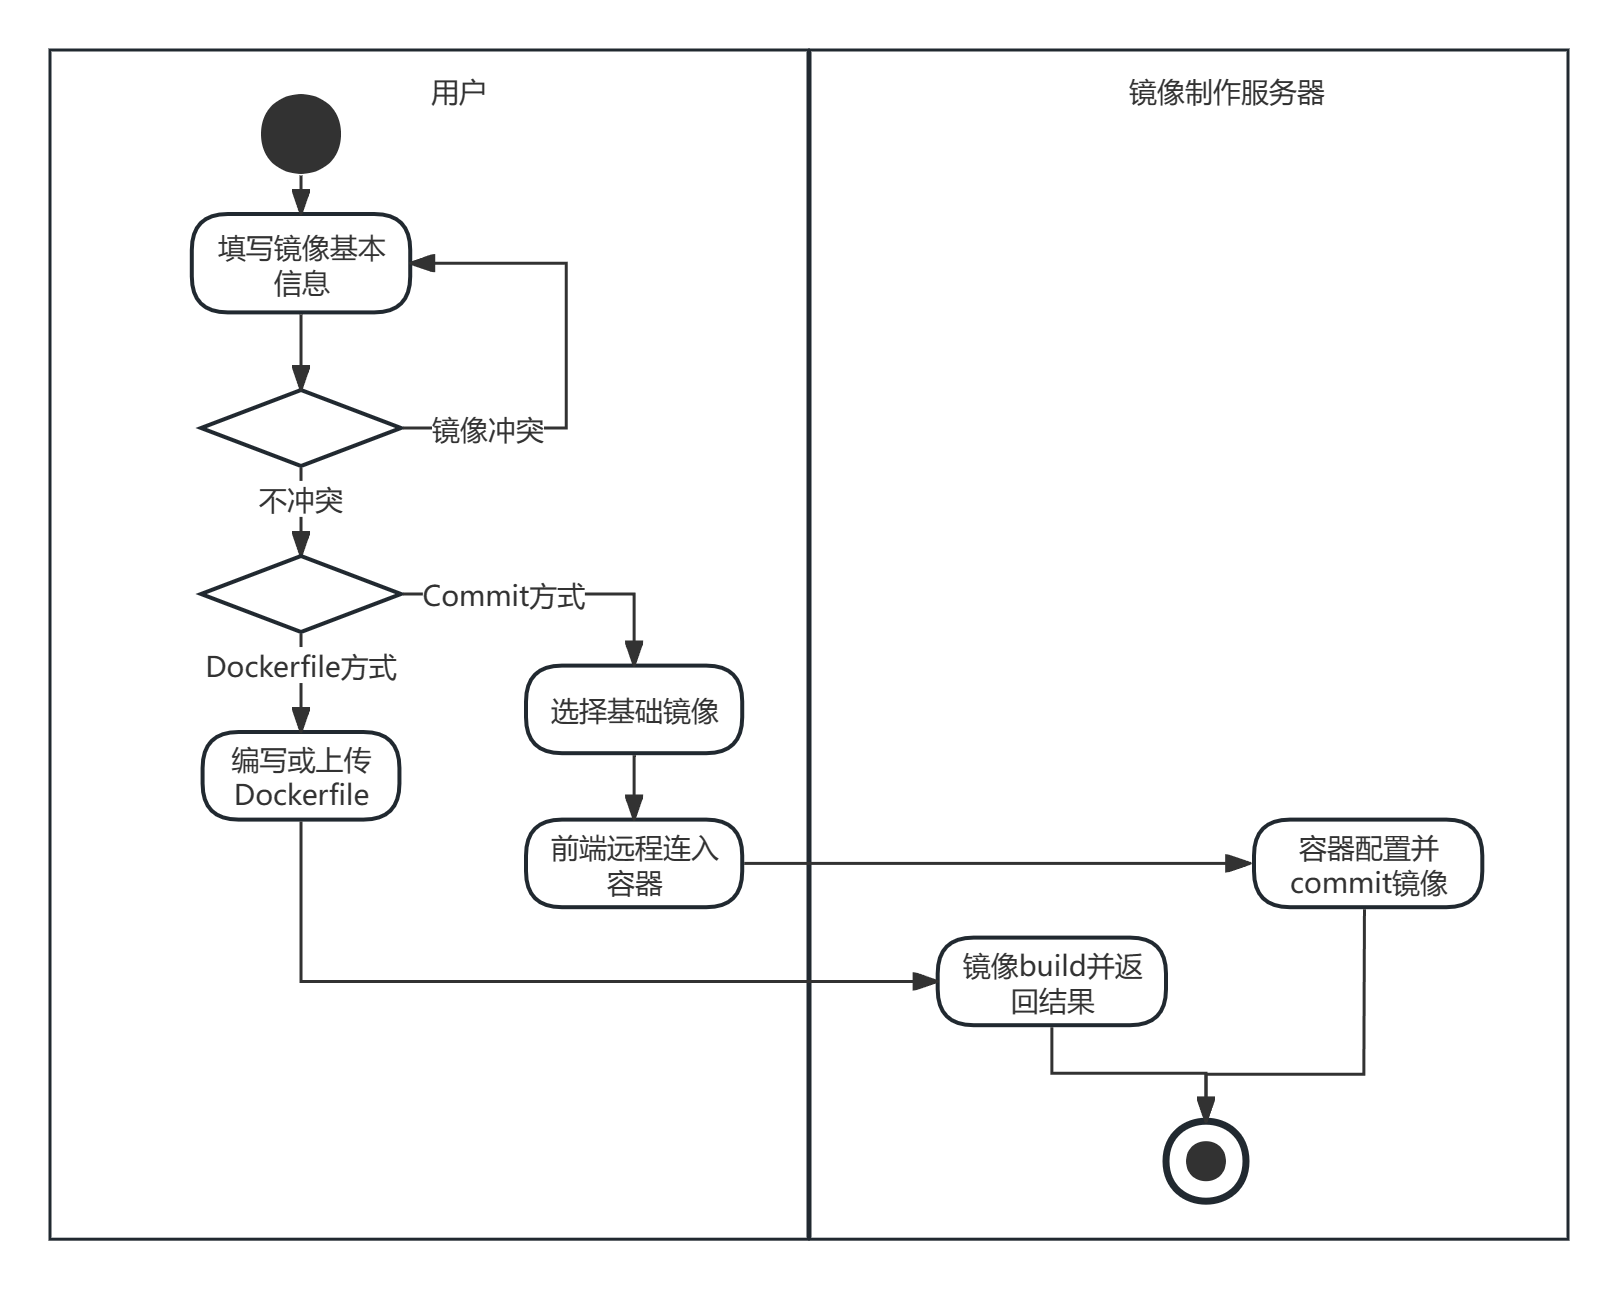
\includegraphics[width=0.8\textwidth]{镜像制作活动图.png}
  \caption{镜像制作活动图}
  \label{fig:镜像制作活动图}
\end{figure}

\subsubsection{镜像删除}

由于系统中需要支持多样的流水线作业,也就势必需要各种各样的镜像。
随着镜像数量的增加,镜像仓库的存储压力也随之上升,因此需要及时清理不再需要的镜像。

尽管Docker官方提供了删除镜像的API,但该API无法清除所有相关文件。
Docker镜像为了节省存储和带宽,采用了分层构建的机制,镜像的每一层都是基于上一层的更改或添加,每一层都是一个单独的文件。
当一个镜像被推送到系统的镜像仓库,每个镜像会拥有一个Manifest文件,这个文件记录了所有组成本镜像所需要的层。
而当调用Docker API删除一个镜像时,只是删除了镜像所对应的Manifest文件,并不会删除其引用的层,这样就导致有些没有被引用的层残留在仓库中。

如图~ \ref{fig:镜像-Manifest文件-层级关系图}所示,有两个镜像分别对应两个Manifest文件,其中Manifest1引用layer1、layer2、layer3,Manifest1引用layer3和layer4。
当我们调用Docker API删除镜像1后,实际上仓库中被删除的只是Manifest1文件,而此时layer4已经不被任何Manifest文件所引用,但却没有被真正删除。

\begin{figure}[h]
  \centering
  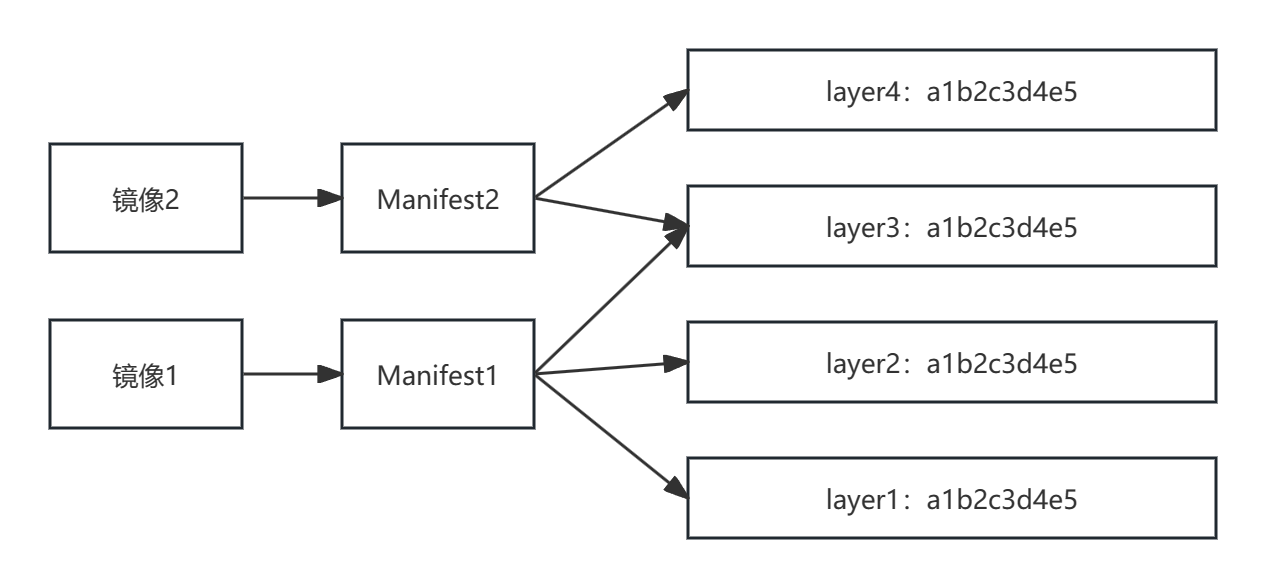
\includegraphics[width=0.8\textwidth]{镜像层级图.png}
  \caption{镜像-Manifest文件-层级关系图}
  \label{fig:镜像-Manifest文件-层级关系图}
\end{figure}

为解决这一问题,系统中引入了引用计数的功能,这一思想在软件工程中经常被运用,如智能指针、垃圾回收等。
系统将为每一个layer维护其引用计数,当某一层的引用次数降至零时,相应的物理文件也会被删除,从而真正释放存储空间。

镜像删除的活动图如图~\ref{fig:镜像删除活动图}所示。

\begin{figure}[h]
  \centering
  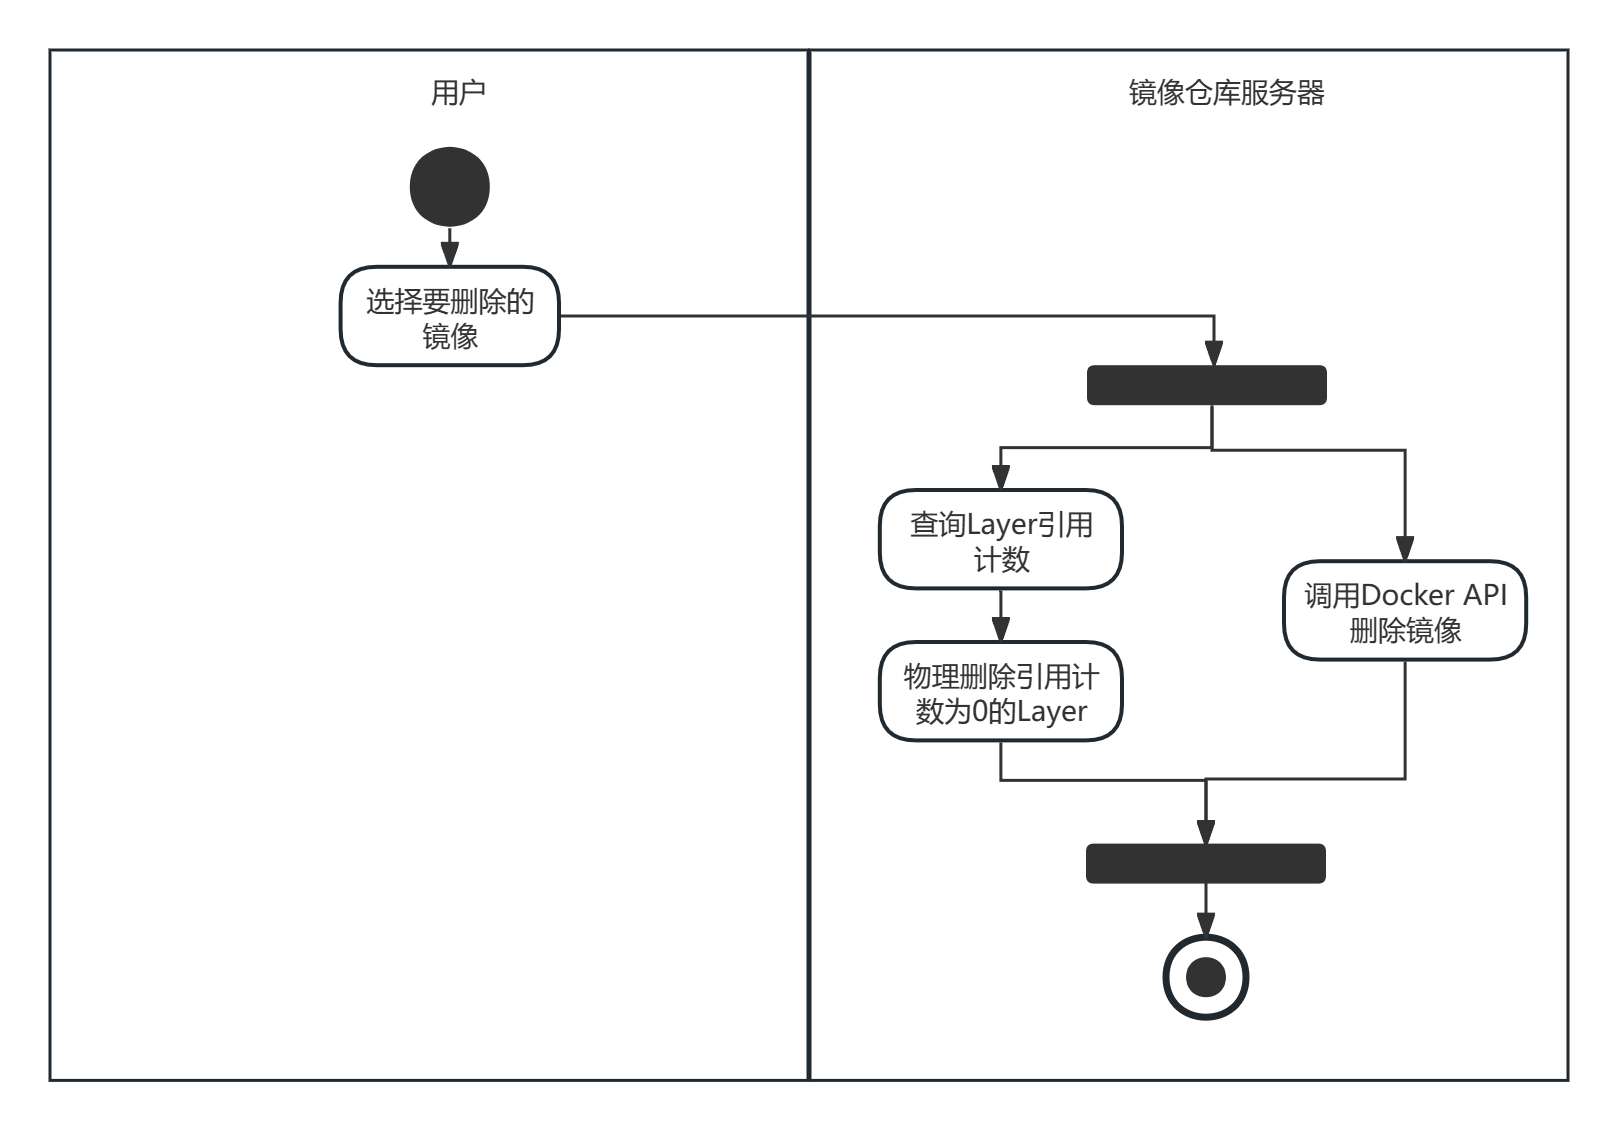
\includegraphics[width=0.8\textwidth]{镜像删除活动图.png}
  \caption{镜像删除活动图}
  \label{fig:镜像删除活动图}
\end{figure}

\subsubsection{镜像上传}
镜像上传功能使用户能够将创建好的镜像推送至仓库中保存。
考虑到镜像移除功能的改进,上传过程中也需要对层引用记录进行相应的更新,以保持系统数据的一致性和完整性。

在上传镜像时,制作服务器调用Docker API推送镜像至仓库。
镜像制作服务器随后通知仓库服务器更新层引用记录文件。
仓库服务器在接收到更新请求后,检查记录文件状态,并据此更新层引用计数。

\subsection{节点管理}
在CI/CD流水线系统中,执行器负责流水线作业的执行,为了满足执行器执行所需的作业的物理与系统环境,执行器所部署的服务器也应有所不同。
节点的本质就是一台物理机或虚拟机,系统使得用户可以自主地对节点进行部署、上下线和删除,以便根据自身作业的需要为其配置所需环境,
对于节点的管理往往同时涉及到数据库节点记录的管理以及对服务器的操作。

\subsubsection{节点注册}
节点注册是系统中对新加入节点进行识别和管理的初步过程。
在设计上,节点注册流程首先需要节点通过调用系统API或通过用户界面手动注册,提交节点的基本信息,如名称、类型(如物理机、虚拟机或Docker)、IP地址、主机名以及任何特定的标签。
这些信息被用于创建节点的唯一标识符(UUID),确保在系统中每个节点都具有唯一性。

注册过程中,系统会校验提交的信息,包括IP地址的格式和可达性、主机名的有效性以及凭证的正确性。
注册成功后,节点的状态被设置为“待部署”,等待后续的一键部署过程完成。
此外,注册流程还包括标签(Tag)管理,一个节点应指定一个或多个标签,这个Tag与创建流水线作业时所指定的Tag是一一对应的,节点中的执行器只会从消息队列中拉取Tag相同的作业进行执行。

\subsubsection{节点一键部署}

节点的一键部署是提升系统效能的关键功能,省去了用户自己去服务器进行执行器部署的步骤。
首先,系统会根据用户提供的IP和部署凭证(用户名、密钥或密码)建立SSH连接,然后创建远程目录,以确保存储配置文件和二进制文件的目录存在,
在此之后备份目标服务器上现有的配置文件,创建或打开新的配置文件和系统ID文件,准备写入新的配置,到此为止,节点部署的准备工作完成。
下载并设置执行器的二进制文件,根据提供的配置,生成执行器的配置文件(config.toml)和系统ID文件,编写并配置执行器的systemd服务文件,以便在系统启动时自动启动执行器。
创建或更新/nix目录,并设置为NFS挂载点(如果需要)。通过systemd管理执行器服务:重新加载systemd守护进程,启用并启动执行器服务,最后关闭SSH连接以释放资源。
如果一切顺利,在执行器成功部署后,该服务器便成为了系统中的一个节点,能够与系统主体进行通信并在该节点上执行流水线作业。

节点一键部署活动图如图~ \ref{fig:节点一键部署活动图}所示。

\begin{figure}[h]
  \centering
  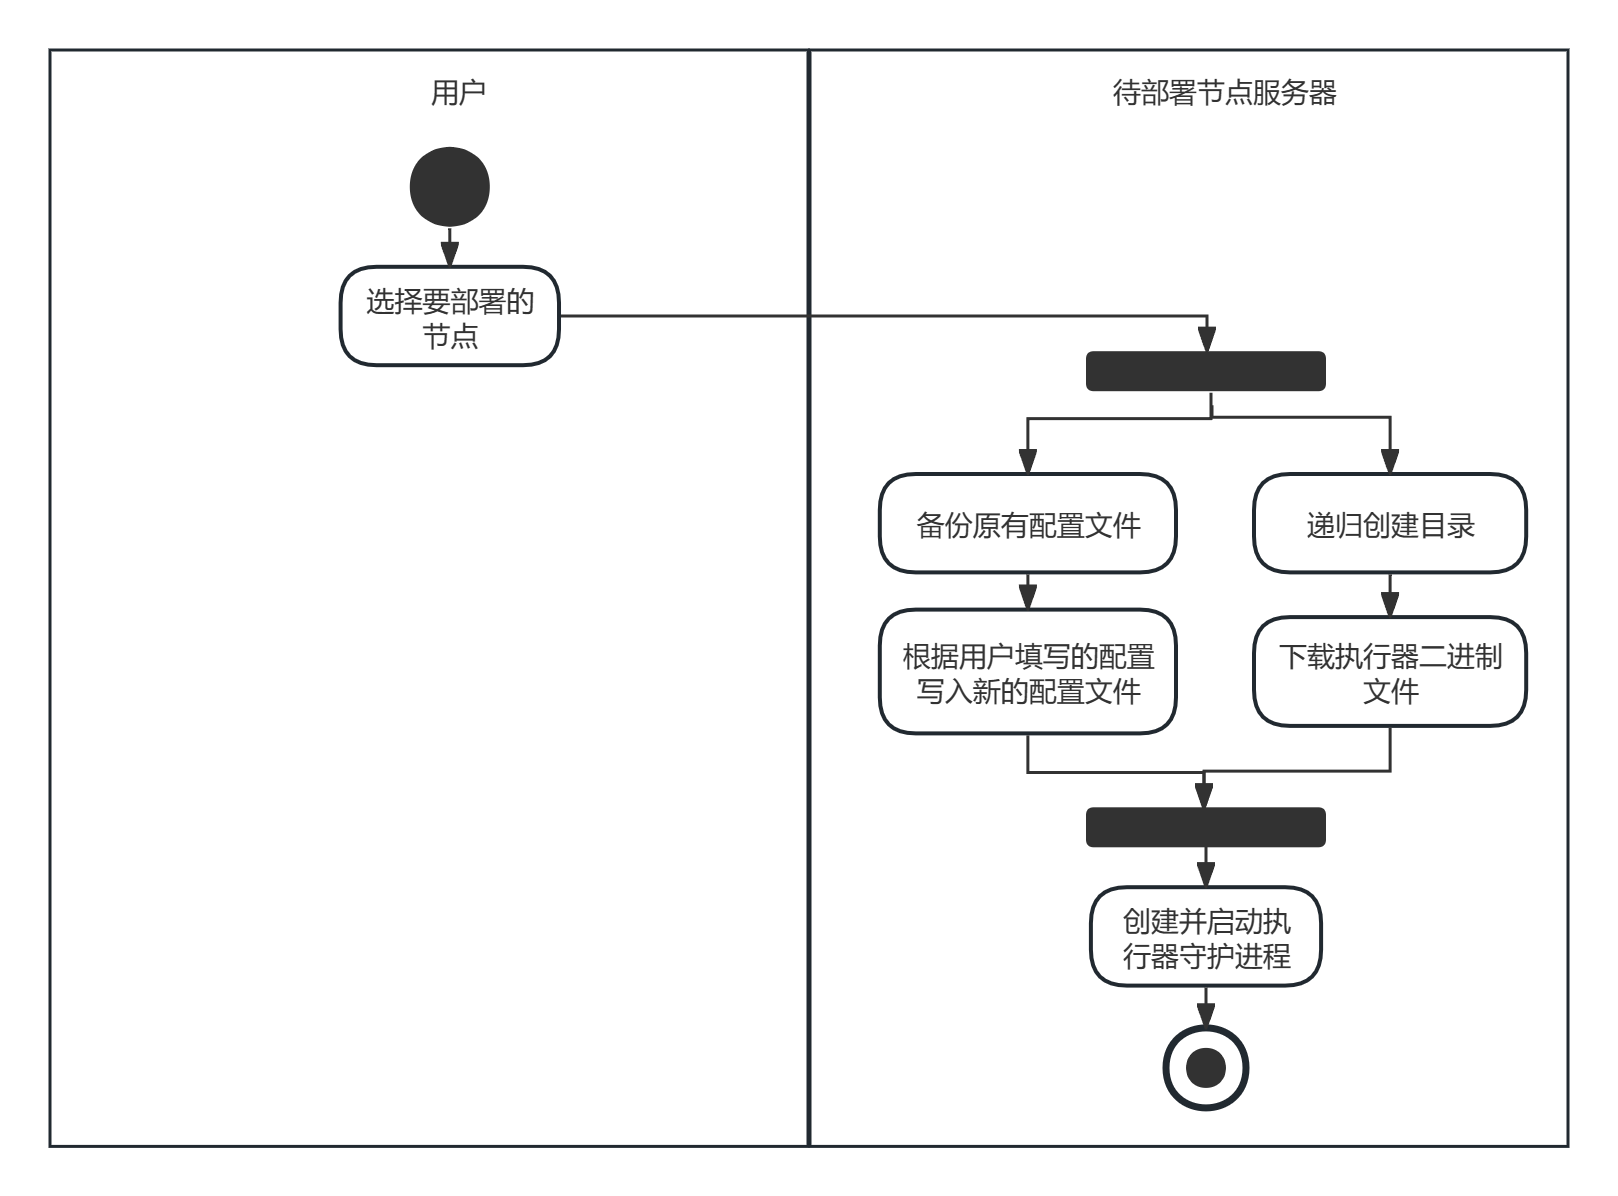
\includegraphics[width=0.8\textwidth]{节点一键部署活动图.png}
  \caption{节点一键部署活动图}
  \label{fig:节点一键部署活动图}
\end{figure}

\subsubsection{节点的上线与下线}
与一键部署同理,在节点的上线与下线过程中,不仅需要在调度系统中更新节点状态,还需要在部署节点的服务器上执行具体的操作以确保这一状态变化得以实际反映。

对于节点上线来说,首先需要SSH连接到节点服务器,使用systemctl start命令启动节点注册时配置好的执行器服务。
此后需要进行必要的健康检查,包括验证服务进程的状态、测试服务与消息队列和调度器的网络连通性等,
因为节点对应服务器的文件内容和网络状态在节点未上线的过程中,可能会受到其他用户的修改,所以健康检查是确保节点能够成功接收和执行作业,保证节点正常运作的必要步骤。

节点上线的活动图如图\ref{fig:节点上线活动图}所示。

\begin{figure}[h]
  \centering
  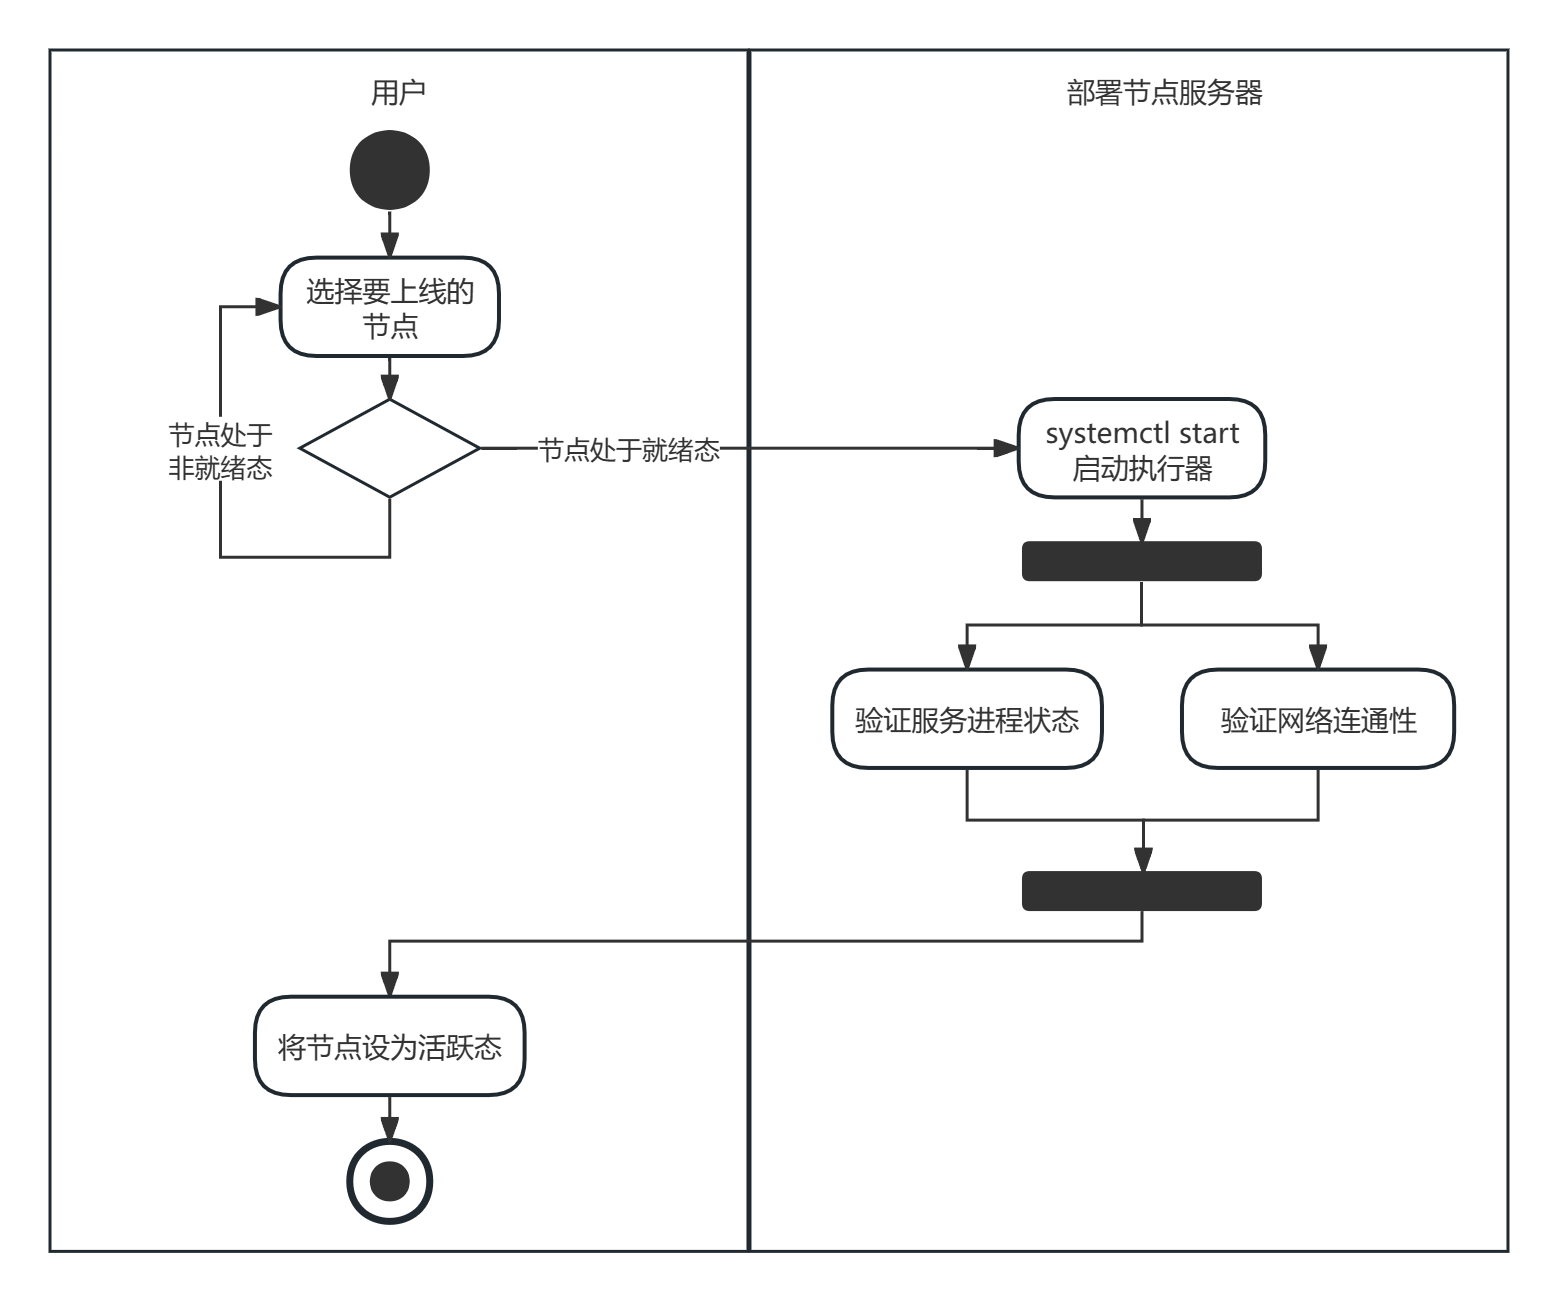
\includegraphics[width=0.8\textwidth]{节点上线活动图.png}
  \caption{节点上线活动图}
  \label{fig:节点上线活动图}
\end{figure}

对于节点下线来说,首先需要安全地停止服务器中的执行器服务,这时如果节点中仍然有执行中的任务,节点将对当前作业进行保持,并将节点设置为待下线的状态,
设置这一状态主要是为了与在线状态进行区分,避免执行完当前任务后又从消息队列中拉取下一任务,导致一直无法下线节点。
待当前作业结束后,进行后处理步骤,首先使用systemctl stop命令停止服务,然后执行必要的清理操作,如临时文件清理和日志上传等,以保证节点下次上线时处于清洁状态,同时减少对相应服务器的磁盘占用。
以上步骤均成功后,节点将被设置为离线状态。

节点下线的活动图如图\ref{fig:节点下线活动图}所示。

\begin{figure}[h]
  \centering
  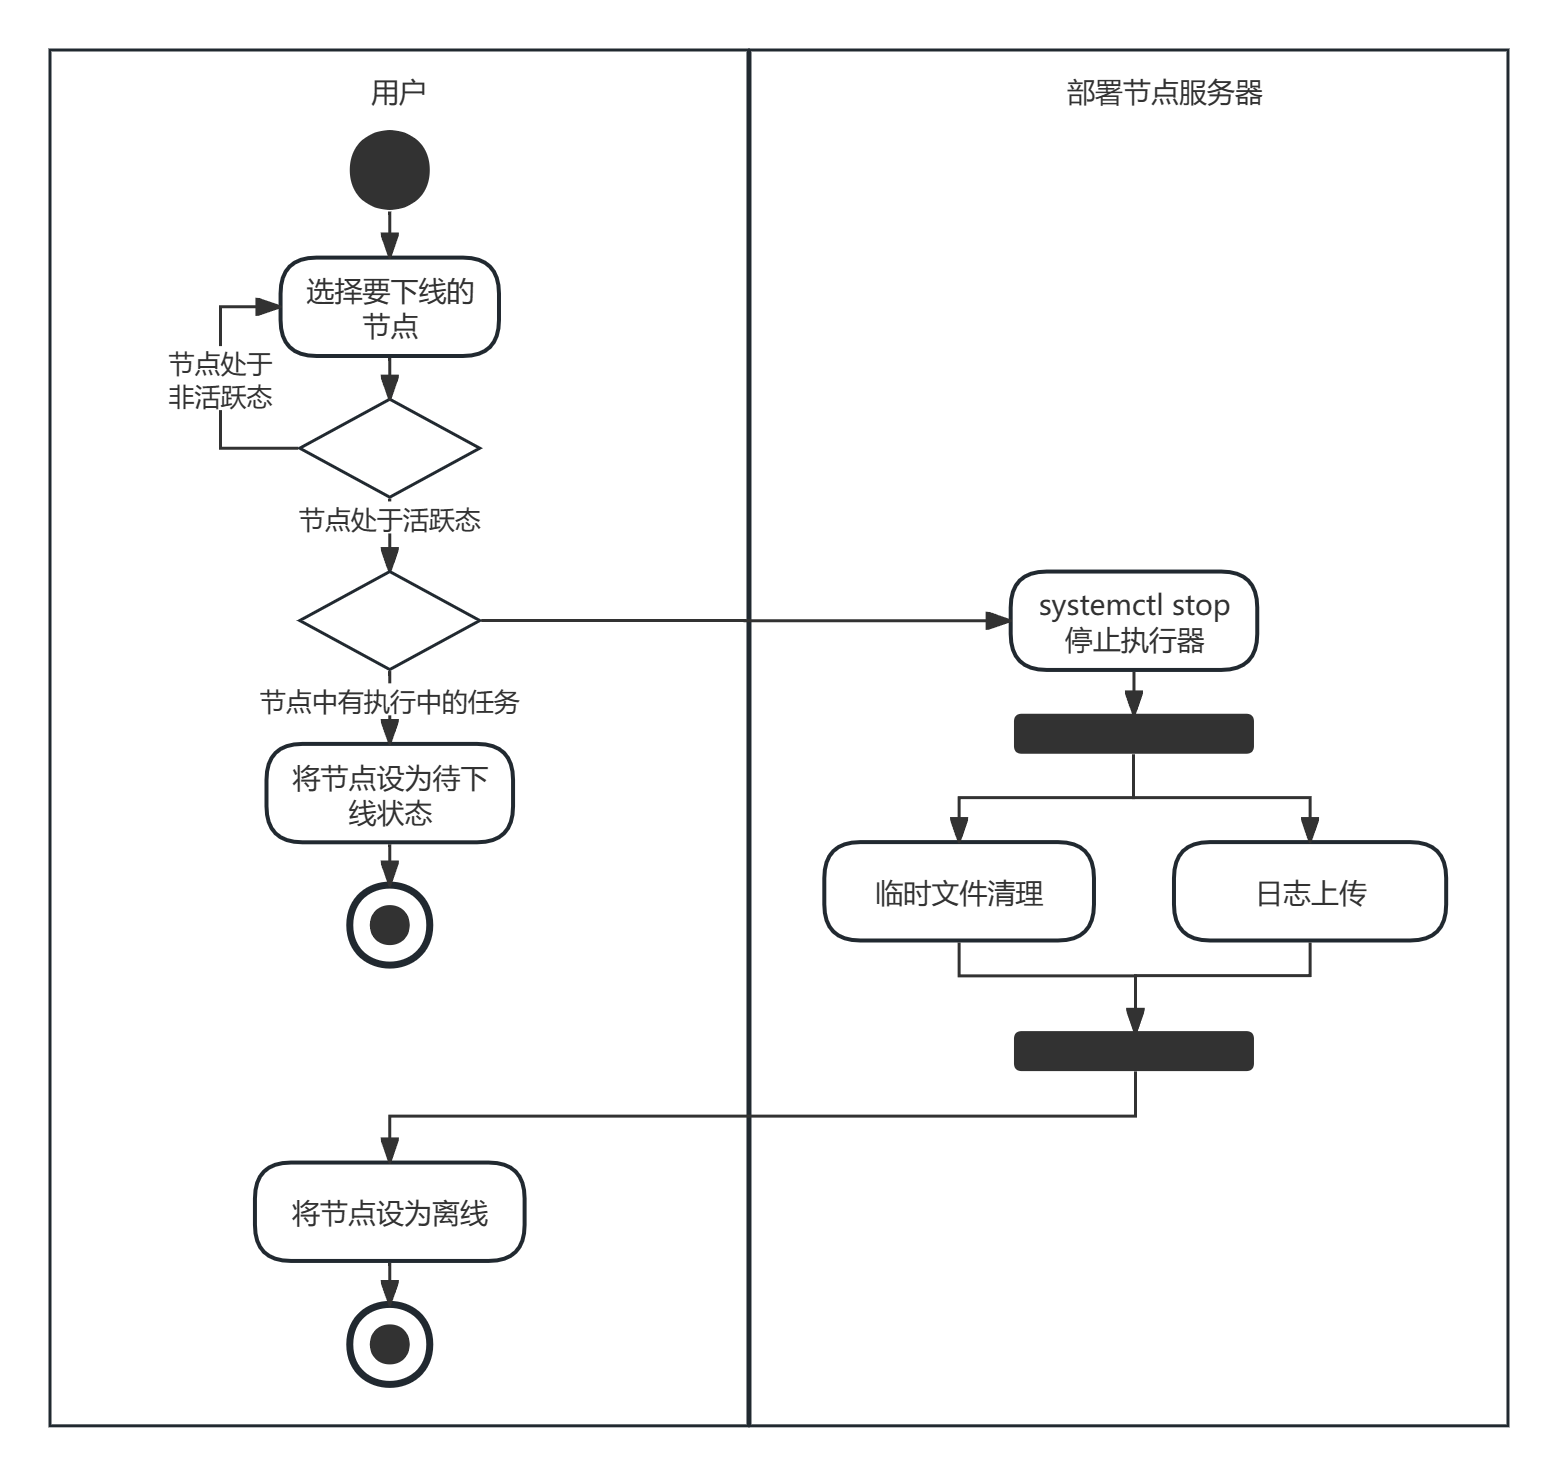
\includegraphics[width=0.8\textwidth]{节点下线活动图.png}
  \caption{节点下线活动图}
  \label{fig:节点下线活动图}
\end{figure}

\subsubsection{节点删除}
节点删除功能允许管理员从系统中彻底移除不再需要的节点,包括数据库记录和部署在服务器上的执行器服务。
删除节点时,首先需要检查节点的状态,如果节点是未部署的状态,直接由Backend模块删除节点的记录即可。
如果是在线或者待下线的状态,则会提示用户无法删除。
如果是离线状态,系统则需要在删除记录的同时,SSH进入服务器中调用执行器的卸载脚本,递归删除执行器的目录。

节点删除的活动图如图\ref{fig:节点删除活动图}所示。

\begin{figure}[h]
  \centering
  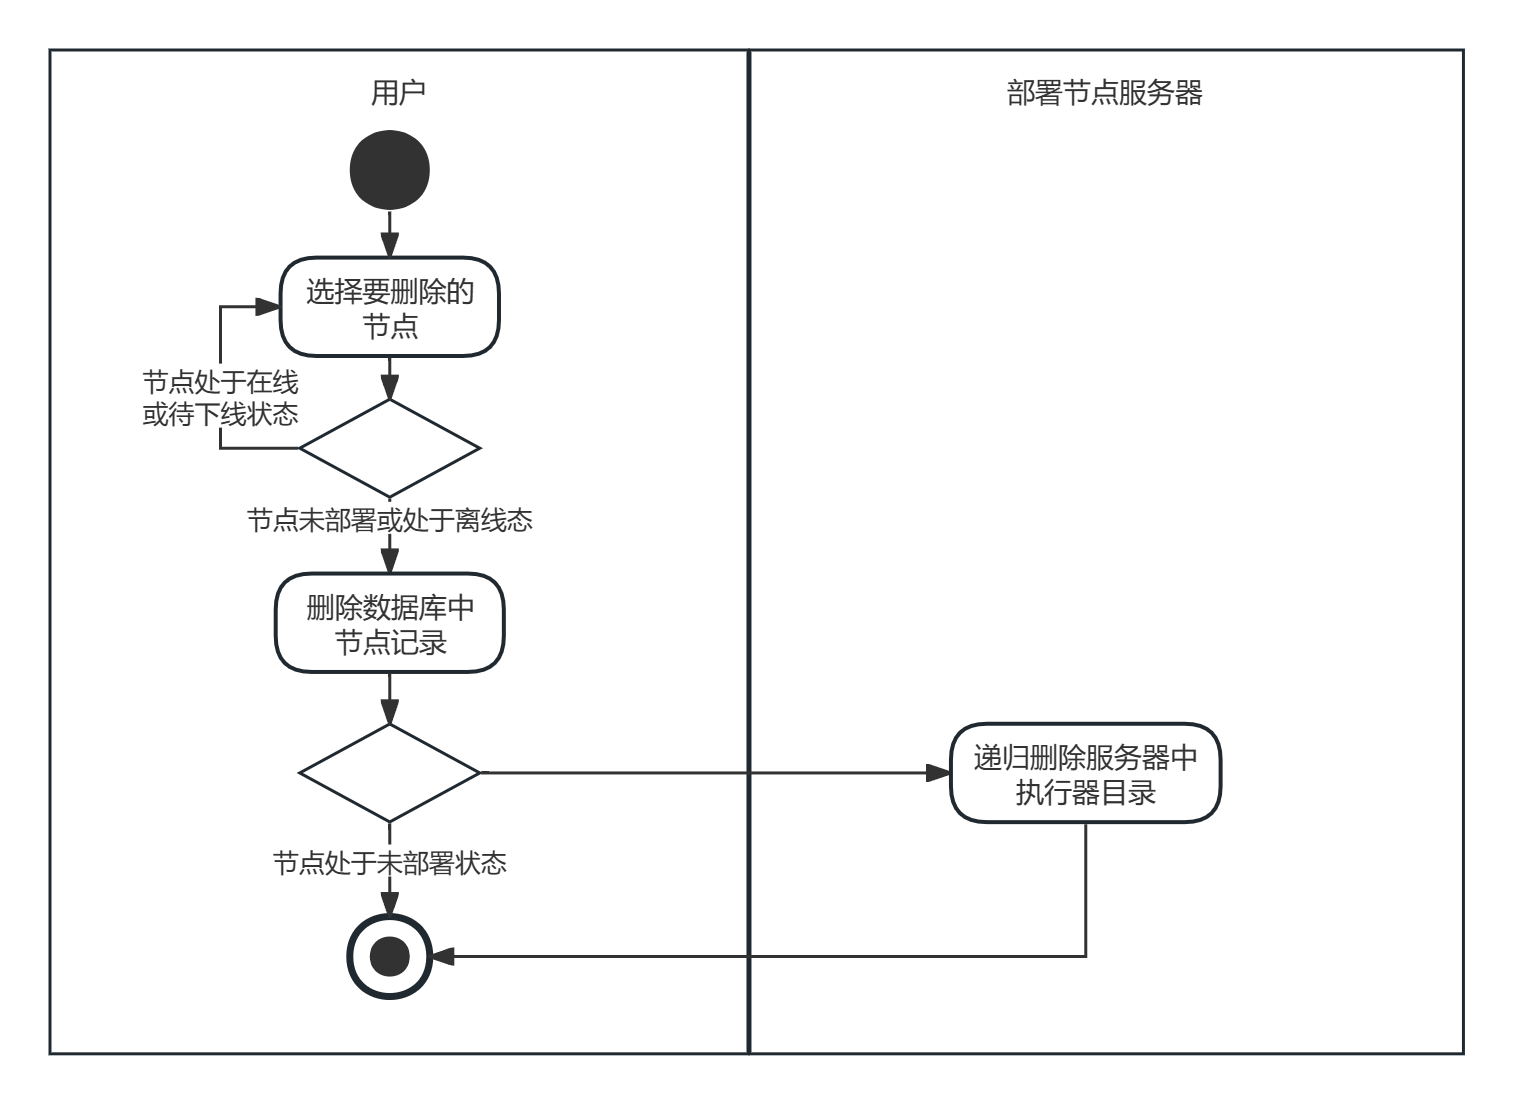
\includegraphics[width=0.8\textwidth]{节点删除活动图.png}
  \caption{节点删除活动图}
  \label{fig:节点删除活动图}
\end{figure}

\section{数据模型设计}
这一部分将系统中的数据进行抽象,从实体、属性和关系三个维度设计出系统的数据模型,并基于此完成了对数据表的设计。

本系统中的与流水线相关的数据实体可以分为两类,一种是配置(Config)相关实体,一种是运行(RunInfo)相关实体。
同时,由于流水线中存在四个不同层级的子概念,所以本系统中可梳理出2×4=8个与流水线相关的实体:
流水线配置、阶段配置、作业配置、任务配置、流水线运行记录、阶段运行记录、作业运行记录、任务运行记录。

同时,根据前文对需求的整理和分析,系统中还需要对镜像和节点两个概念进行抽象,而节点又是根据Tag标签的方式与作业进行联系的。
所以系统中还应有镜像、节点和节点标签三个实体,加上流水线相关实体,共11个实体。

接下来对实体中的主要属性进行分析,由于流水线相关实体较多且内容具有相似性,此处选取代表性的“作业”相关实体进行分析。

对于作业配置相关实体,应主要包含以下几个方面的属性:
基本信息类包括作业id(主键)、作业所属的阶段id(外键)、名称、创建时间、修改时间、作业位于阶段中的位置;
构建信息类包括,包括 Docker 镜像、输入环境变量;
执行信息类包括:超时时间、触发类型(自动/人工/定时)、是否启用。
可以得到数据库中作业配置表如表~ \ref{tab:作业配置表}

\begin{table}[h]
  \centering
  \caption{作业配置表}
  \label{tab:作业配置表}
  \begin{tabular}{cll}
    \toprule
    字段名                  & 类型            & 描述                                       \\
    \midrule
    id                      & Char           & 主键id                                   \\
    name                    & Char           & 作业名称                                   \\
    trigger\_type           & Char           & 触发方式,自动/手动                        \\
    stage\_config\_id       & ForeignKey     & 关联的阶段配置                             \\
    created\_at             & DateTime       & 创建时间                                    \\
    updated\_at             & DateTime       & 更新时间                                    \\
    image\_id               & ForeignKey     & 关联的Docker镜像                            \\
    variables               & JSON           & 未赋值环境变量                              \\
    tag                     & Char           & 标签                                       \\
    timeout                 & Integer        & 超时时间                                    \\
    position                & Integer        & 位置                                        \\
    run\_condition          & Char           & job的运行条件                               \\
    active                  & Boolean        & 是否启用                                    \\
    version                 & Integer        & 版本号,以追溯修改历史                        \\
    \bottomrule
  \end{tabular}
\end{table}

对于运行记录相关实体,以作业运行记录为例,应包含以下几个方面的属性:
基本信息类包括作业运行记录id(主键)、作业运行记录所属的阶段运行记录id(外键)、作业运行记录所属的作业id(外键);
触发信息类:触发时间、触发人、触发类型;
运行信息类:开始时间、结束时间、作业状态、赋值后的环境变量;
可以得到数据库中作业运行记录表如表~ \ref{tab:作业运行记录表} 所示。

\begin{table}[h]
  \centering
  \caption{作业运行记录表}
  \label{tab:作业运行记录表}
  \begin{tabular}{cll}
    \toprule
    字段名               & 类型          & 描述                                               \\
    \midrule
    job\_config\_id     & ForeignKey   & 关联的作业配置                                     \\
    stage\_run\_info\_id    & ForeignKey   & 关联的阶段运行信息                                 \\
    started\_at         & DateTime     & 作业运行开始时间                                   \\
    end\_at             & DateTime     & 作业运行结束时间                                   \\
    repo\_url           & Char         & 代码仓库URL                                      \\
    repo\_branch        & Char         & 分支名                                           \\
    ref\_sha            & Char         & commit id                                       \\
    variables           & JSON         & 赋值后的环境变量                                  \\
    state               & Char         & 作业的状态,如pending/running/success等            \\
    selected            & Boolean      & 触发时是否勾选,布尔值                             \\
    \bottomrule
  \end{tabular}
\end{table}

其余的流水线配置、阶段配置与任务配置中的属性与作业配置大同小异,此处不再赘述。

然后分析镜像、节点和节点标签三个实体。
对于Docker镜像,有镜像名、镜像ID、镜像描述等基本信息,同时应有镜像标签(Image Label)镜像地址等与镜像存储相关的属性;
节点的本质是一个服务器,应包含服务器信息,如服务器IP、端口号、主机名、登录凭证等,同时也应包含节点名称、节点描述等基本信息。
节点标签是不同作业分配到不同节点上的依据,同时又是节点与作业多对多关系的中间表,包含名称、节点ID、作业ID等属性。

最后分析系统内实体之间的关系。一个配置的一次执行即产生了一个运行实例,这与编程语言中“类”和“类对象”的关系类似,
即“运行”是“配置”的实例化,“配置”是“运行”的模板,因此配置与运行是一对多的关系。
同时根据流水线的各个子概念的定义,我们知道有:流水线与阶段是一对多的关系,阶段与作业是一对多的关系,作业与任务是一对多的关系。
由于作业中包含镜像,所以镜像与作业是一对多的关系。每个作业需要指定一个节点或多个节点,每个节点又可以被多个作业所指定,所以作业与节点是多对多的关系,作业标签自然就是作业与节点的中间表。

结合以上分析,可得出系统的实体-关系图(E-R图)如图~\ref{fig:系统E-R图}:

\begin{figure}[h]
  \centering
  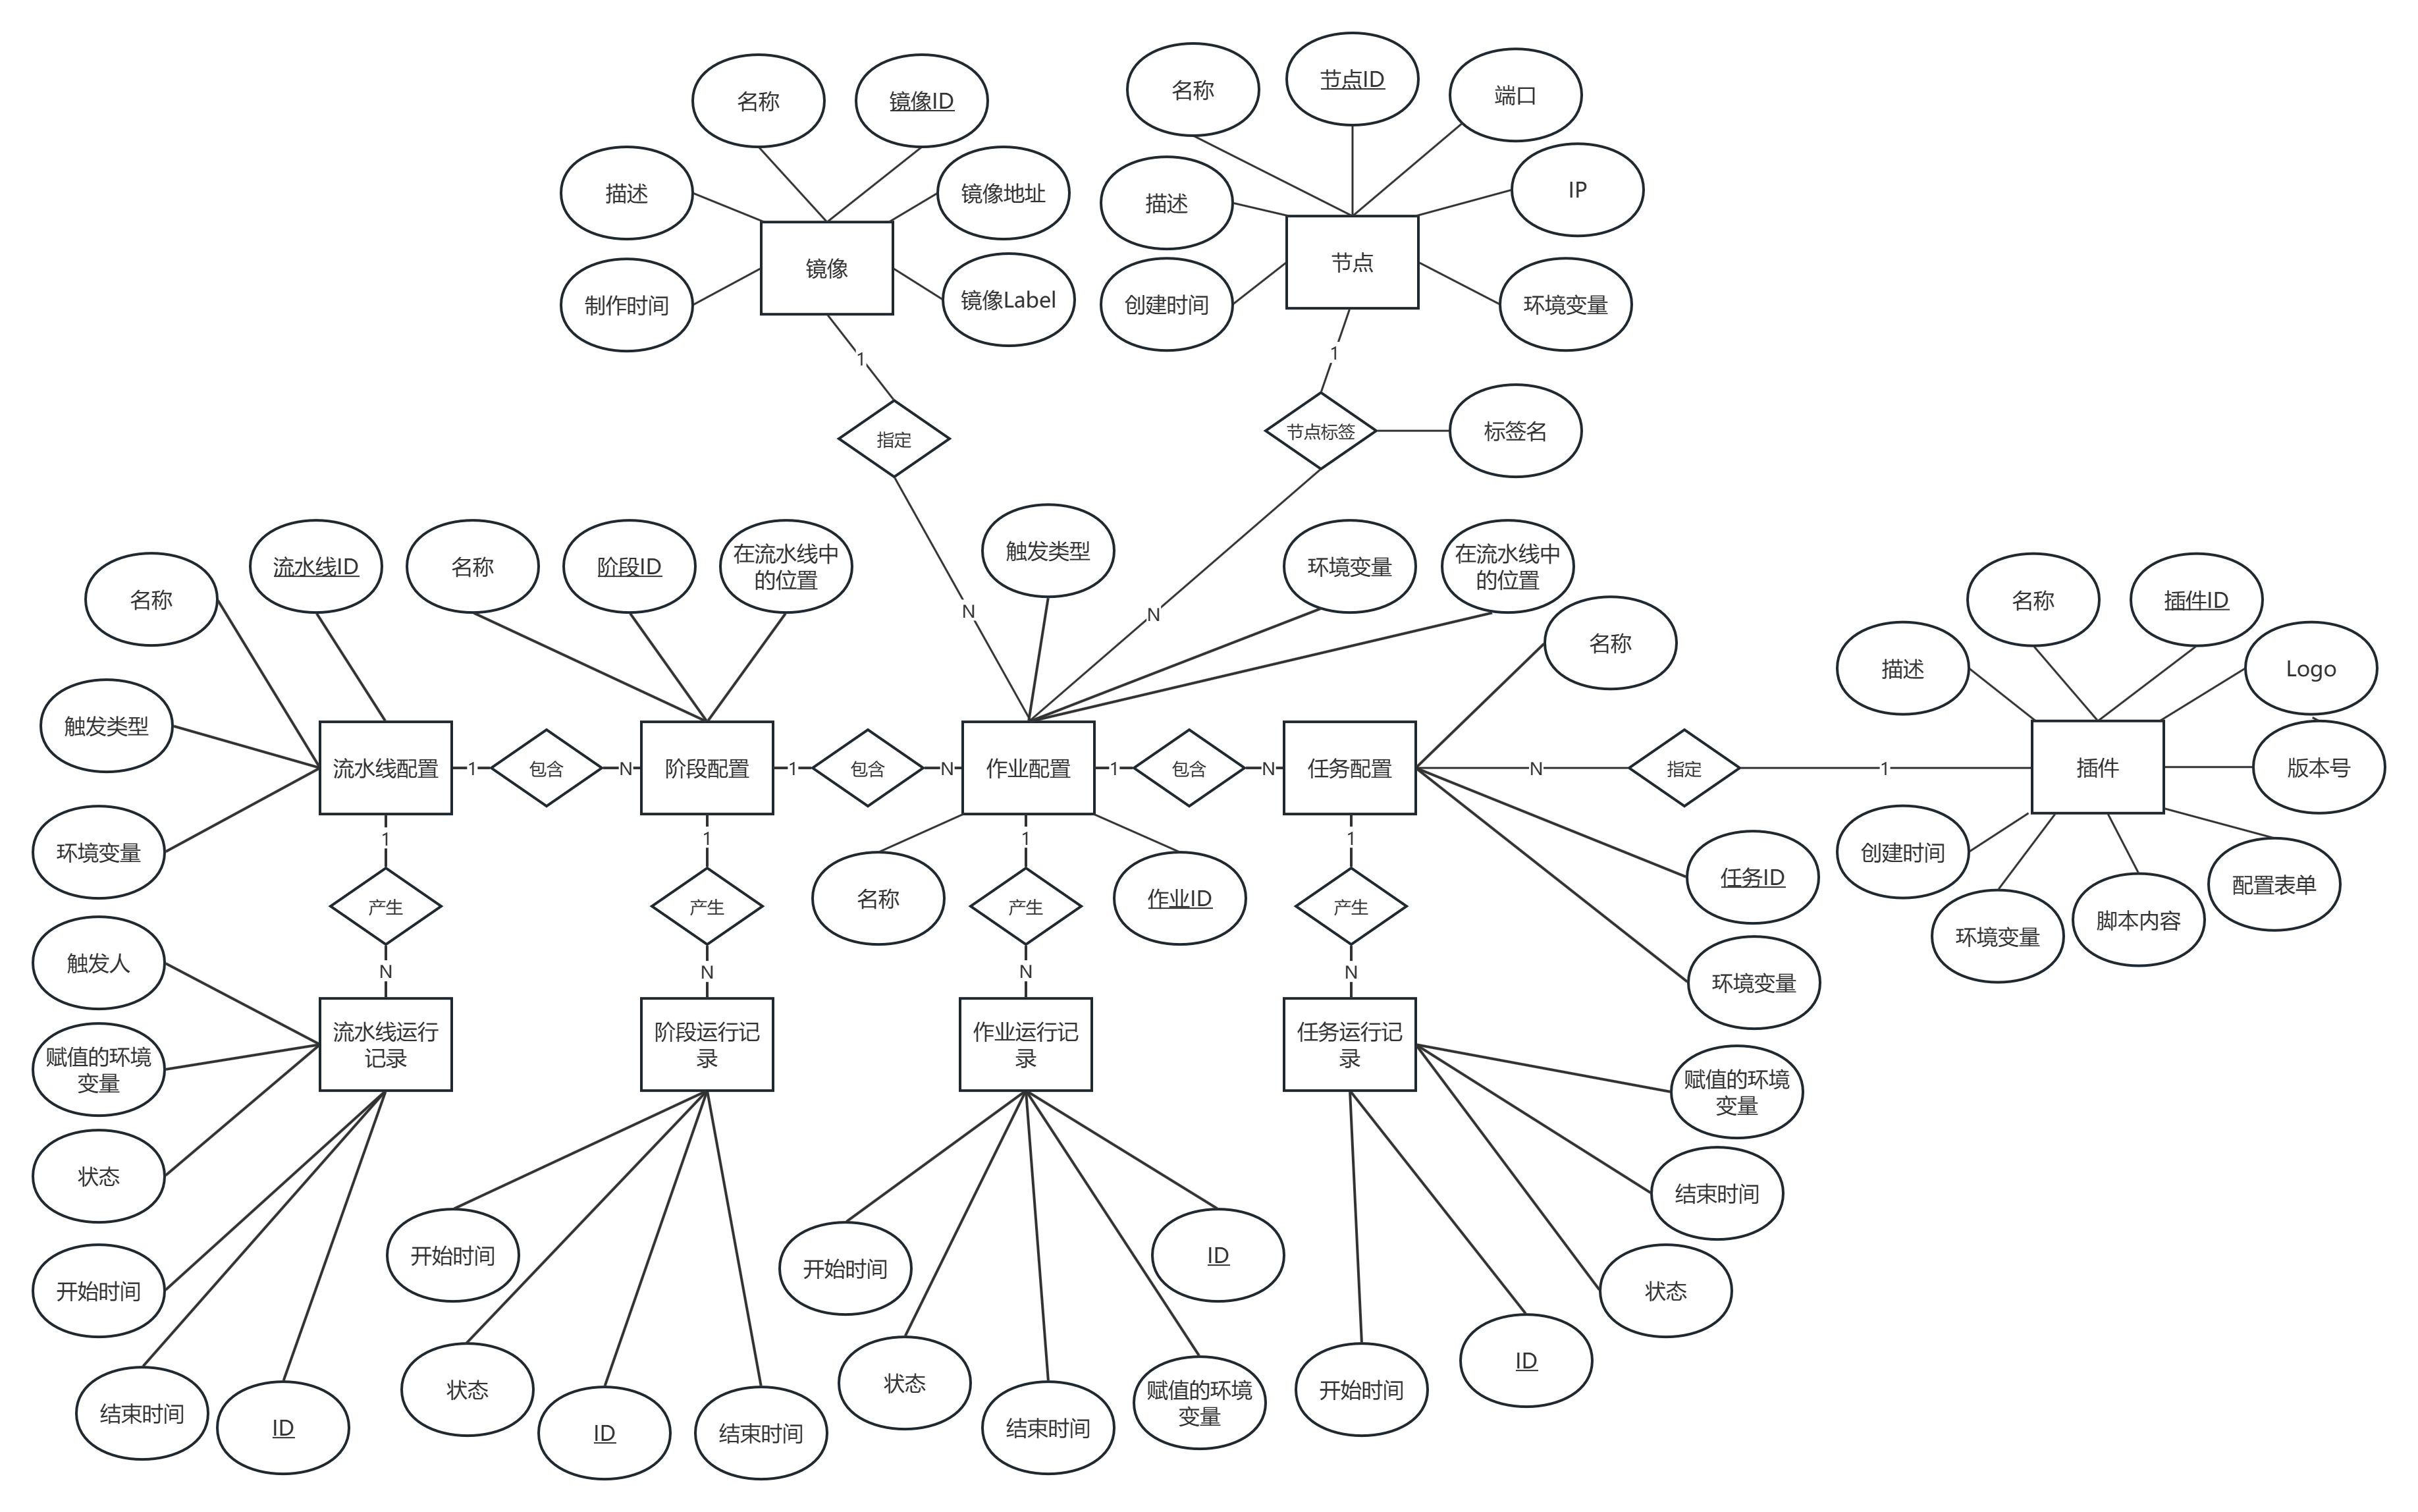
\includegraphics[width=1\textwidth]{系统ER图.png}
  \caption{系统E-R图}
  \label{fig:系统E-R图}
\end{figure}


